\documentclass[sigconf]{acmart}
\settopmatter{printfolios=true,printccs=true,printacmref=true}
\linespread{0.98}



%%%%%%%%%%%%%%%%%%%%%%%%%%% For ICSE '20 %%%%%%%%%%%%%%%%%%%%%%%%%%%%%%%
\setcopyright{acmcopyright}
\acmDOI{10.1145/3377811.3380428}
\acmISBN{978-1-4503-7121-6/20/05}
\acmYear{2020}
\copyrightyear{2020}
\acmPrice{15.00}
\acmConference[ICSE '20]{42nd International Conference on Software Engineering}{May 23--29, 2020}{Seoul, Republic of Korea}
\acmBooktitle{42nd International Conference on Software Engineering (ICSE '20), May 23--29, 2020, Seoul, Republic of Korea}
%%%%%%%%%%%%%%%%%%%%%%%%%%% For ICSE '20 %%%%%%%%%%%%%%%%%%%%%%%%%%%%%%%




%%%%%%%%%%%%%%%%%%%%%%%%%%%%%%%%%%%%%%%%%%%%%%%%%%%%%%%%%%%%%%%%%%%

%\usepackage{algorithm}        % for algorithm (float) environment
\usepackage[linesnumbered,ruled]{algorithm2e}
\makeatletter
\renewcommand{\@algocf@capt@plain}{above}% formerly {bottom}
\makeatother
\usepackage{algorithmicx}
\usepackage{algpseudocode}    % for algorithmic
\usepackage{amsmath}
\usepackage{amssymb}

%\usepackage{authblk}
%\usepackage[utf8]{inputenc}
%\usepackage[T1]{fontenc}

\usepackage{balance}
\usepackage{bbding}
\usepackage{booktabs}
\usepackage{calc}
\usepackage{circuitikz}
\usepackage{color}            % for note colors
\usepackage{etex}
\usepackage{filecontents}
\usepackage{graphicx}
\usepackage[customcolors]{hf-tikz}
\usepackage{listings}
\usepackage{mdwlist}          % Compact \itemize*, \enumerate*
\usepackage{microtype}        % better hyphenation
\usepackage{multirow}
\usepackage{paralist} % for compactitem
\usepackage{pgfplots}
\usepackage{pifont}
\usepackage{pst-circ}
\usepackage{pstricks}
\usepackage{relsize}
\usepackage{setspace}
\usepackage{stmaryrd}
\usepackage{subfigure}
\usepackage[T1]{fontenc}      % T1 enconding
\usepackage{tikz}
\usepackage[utf8]{inputenc}   % use UTF-8
\usepackage[USenglish]{babel} % US English hyphenation rules
\usetikzlibrary{matrix,arrows,positioning,shapes,backgrounds,fit}
\pgfplotsset{compat=1.3}
\usepackage{wasysym}
\usepackage{xcolor}

\newcommand\ignore[1]{}
\newcommand{\highlight}[1]{\vspace{.15cm}\noindent\textcolor{blue}{\textbf{#1}}}
\newcommand{\textcode}[1]{\texttt{#1}}
%\newtheorem{definition}{Definition}

\newcommand*\circled[1]{\tikz[baseline=(char.base)]{
				\node[shape=circle,draw,inner sep=1pt] (char) {\scriptsize{#1}};}}

\newcommand{\Command}{Operation }
\newcommand{\Commands}{Operations }
\newcommand{\command}{operation }
\newcommand{\commands}{operations }
\newcommand{\Operation}{Event }
\newcommand{\Operations}{Events }
\newcommand{\operation}{event }
\newcommand{\operations}{events }

\newcommand{\Var}{\mathit{V}}
\newcommand{\SVar}{\mathit{SV}}
\newcommand{\LVar}{\mathit{LV}}
\newcommand{\WVar}{\mathit{WV}}
\newcommand{\lval}{\mathit{lval}}
\newcommand{\fork}{\mathit{fork}}
\newcommand{\join}{\mathit{join}}
\newcommand{\Loc}{\mathit{Loc}}
\newcommand{\Active}{\mathit{A}}
\newcommand{\Val}{\mathit{Val}}
%\newcommand{\edge}[1]{\stackrel{#1}{\longrightarrow}}
\newcommand{\edge}[1]{\xrightarrow{#1}}
\newcommand{\Code}{\mathit{Code}}
\newcommand{\Result}{\mathit{Result}}

\newcommand{\test}{\mathit{test}}
\newcommand{\tests}{\mathit{tests}}
\newcommand{\newTests}{\mathit{newTests}}
\newcommand{\mem}{\textsf{Mem}}
\newcommand{\pcon}{\mathit{pc}}
\newcommand{\instr}{\mathit{instr}}
\newcommand{\Instr}{\mathit{Instr}}
\newcommand{\Transition}{\mathit{T}}
\newcommand{\Inputs}{\mathit{I}}
\newcommand{\Location}{\mathit{L}}

%\algrenewcommand\alglinenumber[1]{\scriptsize #1:} % change the pseudocode line number size
\newcommand{\NewST}{\State\textcolor{darkblue}}
\newcommand{\NewSTX}{\Statex\textcolor{darkblue}}
%\newcommand{\qed}{$\diamond$}
\newcommand{\outline}[1]{}

\newcommand{\SpecuSym}{\textsc{SpecuSym} }
\newcommand{\SymExec}{\textsf{BaseSymExec} }

\let\oldnl\nl% Store \nl in \oldnl
\newcommand{\nonl}{\renewcommand{\nl}{\let\nl\oldnl}}% Remove line number for one line

%%%%%%%%%%%%%%%%%%%%%%%%%%%%%%%%%%%%%%%%%%%%%

%%%%%%%%%%%%%%%%%%%%%%%%%%%%%%%%%%%%%%%%%%%%%minglingh
% temporal logic formulae
%
\newcommand{\AG}{\textbf{AG }}
\newcommand{\AF}{\textbf{AF }}
\newcommand{\EF}{\textbf{EF }}
\newcommand{\EX}{\textbf{EX }}
%
\newcommand\api[1]{\texttt{\hyphenchar\font=`-#1}}
\newcommand\var[1]{\texttt{\hyphenchar\font=`-#1}}
\newcommand\mytexttt[1]{\texttt{\hyphenchar\font=`-#1}}
%
\newcommand{\aut}[1]{\mathcal{#1}}
\newcommand{\proc}[1]{\textsc{#1}}

\newcommand{\prog}{\mathcal{P}}
\newcommand{\cove}{\mathcal{C}}
\newcommand{\testI}{\mathcal{I}}
\newcommand{\testS}{\mathcal{S}}

\newcommand{\STEM}{\mathcal{A}}

\newcommand{\eval}{\mathit{eval}}
\newcommand{\true}{\mathsf{true}}
\newcommand{\false}{\mathsf{false}}
\newcommand{\pfx}{\mathsf{pfx}}
\newcommand{\first}{\mathsf{first}}
\newcommand{\last}{\mathsf{last}}
\newcommand{\assume}{\mathsf{assume}}
\newcommand{\assert}{\mathsf{assert}}
\newcommand{\lock}{\mathit{lock}}
\newcommand{\unlock}{\mathit{unlock}}
\newcommand{\acquire}{\mathit{sem\_wait}}
\newcommand{\release}{\mathit{sem\_post}}

\newcommand{\mbeq}{\overset{!}{=}}
%%%%%%%%%%%%%%%%%%%%%%%%%%%%%%%%%%%%%%%%%%%%%

\definecolor{darkblue}{rgb}{0, 0.125, 0.576}
\definecolor{dkgreen}{rgb}{0,0.6,0}
\definecolor{gray}{rgb}{0.5,0.5,0.5}
\definecolor{mauve}{rgb}{0.58,0,0.82}

\lstset{frame=tb,
  language=C,
  aboveskip=3mm,
  belowskip=3mm,
  showstringspaces=false,
  columns=flexible,
  basicstyle={\scriptsize\ttfamily},
  numbers=none,
  numberstyle=\tiny\color{gray},
  keywordstyle=\color{blue},
  commentstyle=\color{dkgreen},
  stringstyle=\color{mauve},
  breaklines=true,
  breakatwhitespace=true,
  tabsize=3,
  numbers=left, % where to put the line-numbers; possible values are (none, left, right)
  numbersep=5pt
}


\newcommand{\HB}[1]{\textcolor{blue}{Huibo}{\textcolor{red}{#1}}}
% Author's notes  (remember to comment out before submission)
\newcommand\sgnote[1]{\textcolor{blue}{{\textbf{Daniel Says: #1}}}}
\newcommand\mwnote[1]{\textcolor{red}{{\textbf{Meng Says: #1}}}}
\newcommand\plnote[1]{\textcolor{green}{{\textbf{Peng Says: #1}}}}
%

%%%%%%%%%%%%%%%%%%%%%%%%%%%%%%%%%%%%%%%%%%%%%
%
% formatting source code
%
\newcommand{\Ind}[1]{\hspace{#1ex}\hspace{#1ex}\hspace{#1ex}}

%\newcommand{\textcode}[1]{\texttt{\small #1}}
%\newcommand{\highlight}[1]{\vspace{.15cm}\noindent\textbf{#1}}
\newcommand{\submissioncomment}[1]{  }

\newtheorem{observation}{Observation}
%\newtheorem{definition}{Definition}
%\newtheorem{theorem}{Theorem}
%\newtheorem{example}{Example}
%\newtheorem{thrm}{Theorem}
%\newtheorem{lem}{Theorem}
%\newtheorem{defn}{Definition}
\newtheorem{pro}{Property}

% Some tikz shapes to draw cool stuff
\definecolor{salmon}{RGB}{255,191,191}
\tikzset{
  woval/.style={minglingh
    draw
    , line width=1pt
    %, fill=stree
    , anchor=center
    , text centered
    , rounded corners
  },
}
\tikzset{
  hoval/.style={
    draw
    , line width=1pt
    , fill=salmon
    , anchor=center
    , text centered
    , rounded corners
  },
}
% End tikz shapes

\makeatletter
\newcommand{\setalglineno}[1]{%
  \setcounter{ALG@line}{\numexpr#1-1}}
\makeatother


\begin{document}

\setlength{\abovedisplayskip}{3pt}
\setlength{\belowdisplayskip}{3pt}

\title[]{\textsc{SpecuSym}: Speculative Symbolic Execution for Cache Timing Leak Detection}


\author{Shengjian Guo}
\authornote{Both authors contributed equally to this research.}
\affiliation{%
  \institution{Baidu Security}
}
\email{sjguo@baidu.com}

\author{Yueqi Chen}
\authornotemark[1]
\affiliation{%
  \institution{Penn State University}
}
\email{yxc431@ist.psu.edu}

\author{Peng Li, Yueqiang Cheng}
\authornote{Corresponding author.}
\affiliation{%
  \institution{Baidu Security}
}
\email{{lipeng28,chengyueqiang}@baidu.com}

\author{Huibo Wang}
\affiliation{%
  \institution{Baidu Security}
}
\email{wanghuibo01@baidu.com}

\author{Meng Wu}
\affiliation{%
  \institution{Ant Financial Services Group}
}
\email{bode.wm@antfin.com}

\author{Zhiqiang Zuo}
\affiliation{%
  \institution{State Key Lab. for Novel Software Technology, Nanjing University}
}
%\email{zqzuo@nju.edu.cn}



%\author{Shengjian Guo, Yueqi Chen, Peng Li, Yueqiang Cheng, Huibo Wang, Meng Wu, Zhiqiang Zuo}

%\affiliation{
%\begin{tabular}{cccc}
%  \institution{\baidu~Baidu Security} &
%  \institution{\psu~Penn State University} &
%  \institution{\ant~Ant Financial} &
%  \institution{\nju~Nanjing University}\\
%  \city{Sunnyvale}
%  \state{CA}
%  \postcode{94089}
%  \country{USA} &
%  \textnormal{State College}
%  \state{PA}
%  \country{USA} &
%	\textnormal{Shanghai}
%  \postcode{20000}
%  \country{China} &
%	\textnormal{Nanjing}
%  \state{Jiangsu}
%	\postcode{20000}
%  \country{China} & \\
%  %\textnormal{\{sjguo, lipeng28, yqcheng,hbwang\}@baidu.com} &
%  %\textnormal{yxc431@ist.psu.edu} &
%  %\textnormal{bode.wm@antfin.com} &
%	%\textnormal{zqzuo@nju.edu.cn}
%\end{tabular}
%}

\begin{abstract}
  CPU cache is a limited but crucial storage component in modern processors, 
	whereas	the	cache timing side-channel may inadvertently leak information 
	through the physically measurable timing variances. Speculative execution, 
	a microarchitectural optimization and a source of such variances, can cause 
	severe detriment on deliberate branch mispredictions.
  %
  Despite static analysis could qualitatively verify the timing-leakage-free 
	property under speculative execution, it is incapable of producing endorsements 
	including inputs and speculated flows to diagnose leaks in depth. 
  %
  This work proposes a new method, \textit{Speculative symbolic Execution} 
	(\texttt{SSE}), for precisely detecting cache timing leaks introduced by 
	speculative execution. Given a program (leakage-free in non-speculative 
	execution), \texttt{SSE} systematically explores the program state space, 
	models speculative behavior at conditional branches, and accumulates the	
	cache side effects along with subsequent explorations. 
	%
	During the dynamic execution, \texttt{SSE} constructs leak predicates for 
	memory visits based on the specified cache model and conducts a 
	constraint-solving based cache behavior analysis to generate leak witnesses.
  %
  We have implemented \texttt{SSE} in a tool named \SpecuSym atop KLEE and 
	evaluated it against 15 open-source benchmarks. Experimental results show 
	that \SpecuSym successfully detected leaks in 6 programs upon 4 different 
	cache settings and identified false positives in 2 programs reported by a 
	recent work.
\end{abstract}

\begin{CCSXML}
<ccs2012>
<concept>
<concept_id>10002978.10002979.10002983</concept_id>
<concept_desc>Security and privacy~Cryptanalysis and other attacks</concept_desc>
<concept_significance>500</concept_significance>
</concept>
<concept>
<concept_id>10011007.10011074.10011099</concept_id>
<concept_desc>Software and its engineering~Software verification and validation</concept_desc>
<concept_significance>500</concept_significance>
</concept>
</ccs2012>
\end{CCSXML}
\ccsdesc[500]{Security and privacy~Cryptanalysis and other attacks}
\ccsdesc[500]{Software and its engineering~Software verification and validation}

\keywords{Speculative execution, cache, timing, side-channel leak, symbolic execution} 

\maketitle
\renewcommand{\shortauthors}{S. Guo et al.}


\section{Introduction}
\label{sec:intro}



% First, introduce cache timing side-channel attacks
CPU cache is a limited but crucial storage area on modern processor chips. 
It primarily relieves the speed disparity between the rapid processors and 
the slow main memory, by buffering recently used data for faster reuse. Cache 
timing side-channel attacks~\cite{Kocher96,DhemKLMQW98} leverage the 
distinguishable cache physical symptoms, i.e., the cache visiting latency 
in various program executions, to penetrate the confidentiality of the victim 
system. On exploiting the vulnerable software implementations, adversaries 
are able to extract the application secrets
\cite{OsvikST06,TromerOS10,GullaschBK11,CGM16}, infer the neural network 
structure~\cite{YanFT18,HuLDLXJDLSX18,HongDKLRKDD18,DudduSRB18}, or even 
dump the kernel data
\cite{HundWH13,LippSGPHFHMKGYH18,KocherGGHHLMPSY19,WeisseVMGKPSSWY18}.


% Second, explain timing sc, cache timing sc, and repair; introduce SE 
A timing side channel generally serves as the intermediate carrier through
which private data could be inadvertently disclosed to observers who can 
elaborately measure the timing of certain operations. One particular instance 
is the cache timing side-channel which leaks data by the variance of the 
cache visiting latency. State-of-the-art program repair method~\cite{WuGSW18} 
mitigates cache timing leaks by enforcing constant execution time for all 
secret relevant operations. However, this strong mitigation may still be 
compromised by the thread-level concurrency~\cite{GuoWW18} or the 
instruction-level parallelism like \textit{speculative execution}~\cite{kimuraKT1996}.


% Third, briefly explain SE and its hazard
\textit{Speculative execution}~\cite{kimuraKT1996} is a vital microarchitectural
optimization in modern processors. Essentially, it increases the CPU instruction 
pipeline throughput by beforehand scheduling instructions under predicted branches, 
which prevents control hazards from stalling the pipeline. Despite its importance, 
the cache side effects caused by prediction errors could engender severe detriment 
through the cache timing side channel
\cite{KocherGGHHLMPSY19,BulckMWGKPSWYS18,WeisseVMGKPSSWY18,IslamMBKGES19}. 


% Fourth, reivew the program analysis for SE
Program analysis for speculative execution is by no means a new research domain. 
Literally, existing efforts mainly focused on safe and efficient execution
\cite{ChenLDHY04,PrabhuRV10,GuarnieriKMRS19}, worst case execution time estimation
\cite{LiMR03,LiMR05}, concurrency bug prediction~\cite{ChenWYS09,LiELS05}, and Spectre
vulnerability reasoning~\cite{GuarnieriKMRS19,OleksenkoTSF19,WangCBMR19}, while
Wu et.al~\cite{WuW19} recently proposed static verification of timing-leakage-free 
property under speculative execution. However, such abstract interpretation based 
method~\cite{WuW19} qualitatively answers the \textit{yes} or \textit{no} question 
--- it is incapable of generating input and the speculative flows to diagnose leaks 
in depth. Moreover, the over-approximation nature inevitably leads to false positives, 
which desires a more precise method.



% Fifth, introduce our method 
To this end, we propose a new method, named \textit{speculative symbolic execution}
(\texttt{SSE}), for detecting cache timing leaks introduced by speculative execution. 
Figure~\ref{fig:overall_flow} shows the overall flow of \texttt{SSE}. Given a program 
$\prog$ which is timing-leakage-free under non-speculative execution, the sensitive 
input presented in symbol, and the insensitive input, \texttt{SSE} leverages symbolic 
execution to systematically explores $\prog$'s state space. Meanwhile, it models 
speculative execution at conditional branches (cf. \circled{1}) and accumulates cache 
side effects along with subsequent executions (cf. \circled{2}). Based on a specified 
cache model, \texttt{SSE} constructs leak predicates for memory visits and conducts 
constraint-solving based cache behavior analysis (cf. \circled{3}) to finally generate 
the leak witnesses (cf. \circled{4}). 


\ignore{
To be specific, the symbolic input reflects the leaks that 
are relevant to secret, the speculative execution modeling supplies behavioral 
simulation on program paths, the cache modeling forms leak exposure constraints 
while the the cache analysis discloses divergent cache behaviors at an identified 
execution flow. 
}


% Sixth, point out the challenges 
Our new method has three major challenges. The first challenge comes from the 
modeling of speculative behaviors. Classic symbolic executors
\cite{CadarDE08,PasareanuR10} 
neither support speculative execution nor are cache-aware since they primarily 
concentrates on the functional correctness rather than reasoning the implicit 
program properties. 
%
The second challenge derives from the cache state maintenance. Due to the symbolic 
nature, a symbolic memory address may correspond to multiple concrete addresses. 
Updating the cache status after each memory operation unquestionably leads to an 
explosive number of different cache states. 
%
The last challenge stems from the analysis cost. Processors may trigger multiple 
branch mis-predictions during a program execution. Indiscriminately covering all 
possibilities not only introduces tremendous constraint solving overhead but also 
counts many redundant cases. 


To overcome the first challenge, we design a new modeling algorithm in symbolic 
execution which satisfies both feasibility and high-fidelity. In essence, it 
utilizes the stateful exploration to mimic the speculative behaviors and isolates 
memory changes in auxiliary states from the regular states. 
%
To tackle the second challenge, we develop a lazy modeling strategy which tracks 
memory accesses and lazily reasons about cache effects rather than maintaining a 
complete set of cache states on-the-fly. 
%
To address the last challenge, we filter the branches that are unlikely to cause 
harmful speculative execution. Also, we develop several optimization to shrink 
the constraint size for solving cost reduction.



\ignore{
Also, We develop a merging schema between the mimicked states and regular 
symbolic states to accumulate the cache side effects.

In general, we decompose the precise but lengthy constraint 
into smaller chunks without losing correctness, as well as utilizing 
executor kernel characteristics for faster computation.

However, the side effects caused by speculative execution are normally 
undetectable under standard symbolic execution. To overcome this problem,
we introduce the $\mathit{speculative~modeling}$ into symbolic execution. 
Thus, cache side effects are visible and cache timing leaks from speculative 
execution detectable now. 
}


We have implemented our new method in a prototype named \SpecuSym atop KLEE
\cite{CadarDE08} and LLVM~\cite{LattnerA04} and performed the evaluation on  
15 open-source programs which have 8,791 lines of C code in total. Results 
show that \SpecuSym successfully detects from 22 to 130 leaks in 6 programs 
under 4 set-associative caches and identifies false positives in 2 programs 
reported by recent work.


To summarize, we have made the following contributions:
\begin{compactitem}
  \item 
    A new approach \emph{Speculative Symbolic Execution} for modeling speculative 
		execution and analyzing the affected cache behaviors in symbolic execution.
  \item 
		Implementation of \SpecuSym which addresses the aforementioned challenges
		and supports cache timing leak detection under speculative execution. 
  \item 
    Evaluation of \SpecuSym on 15 open-source benchmarks to demonstrate its 
    effectiveness through discovering from 22 to 130 leaks upon 4 different 
		caches.
\end{compactitem}



\begin{figure}
  \centering
  \scalebox{1.0}{\definecolor{salmon}{RGB}{255,191,191}
\definecolor{leak}{RGB}{255,151,117}
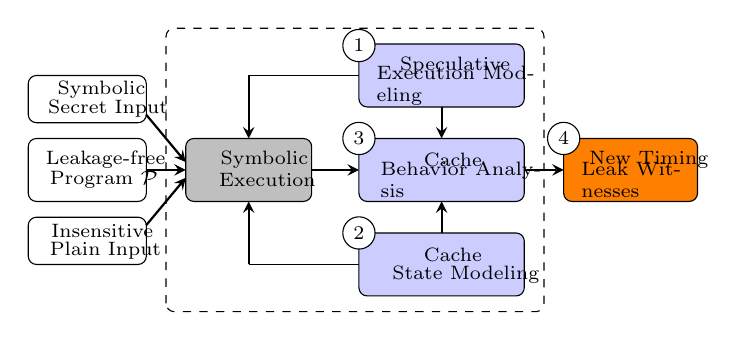
\begin{tikzpicture}[fill=blue!20,font=\scriptsize] 
  \tikzstyle{arrow}=[thick,->,>=stealth,black]
  \tikzstyle{txt}=[above=5pt,right,text width=1.6cm]
  \tikzstyle{long_txt}=[above=5pt,right,text width=2cm]
  \tikzstyle{short_txt}=[above=5pt,right,text width=1.4cm]

  % blocks on left    			
  \draw [rounded corners=3] (0.0, 2.2) rectangle (1.5, 2.8);
  \node [above=5pt,right,text width=1.6cm] at (0.25, 2.45) {Symbolic};
  \node [above=5pt,right,text width=1.6cm] at (0.13, 2.2) {Secret Input};

  \draw [rounded corners=3] (0.0, 1.2) rectangle (1.5, 2.0);
  \node [above=5pt,right,text width=1.6cm] at (0.1, 1.55) {Leakage-free};
  \node [above=5pt,right,text width=1.6cm] at (0.15, 1.3) {Program $\prog$};

  \draw [rounded corners=3] (0.0, 0.4) rectangle (1.5, 1.0);
  \node [above=5pt,right,text width=1.6cm] at (0.17, 0.65) {Insensitive};
  \node [above=5pt,right,text width=1.6cm] at (0.15, 0.4) {Plain Input};

  % line connecting first column and second column
  \draw [arrow](1.5, 2.3)--(2.0, 1.7);
  \draw [arrow](1.5, 1.6)--(2.0, 1.6);
  \draw [arrow](1.5, 0.9)--(2.0, 1.5);
  

  % blocks in the second column
  \draw [fill=lightgray, rounded corners=3] (2.0, 1.2) rectangle (3.6, 2.0);
  \node [txt] at (2.32,1.55){Symbolic};
  \node [txt] at (2.3,1.3){Execution};

  % blocks in the third column
  \draw [fill=blue!20, rounded corners=3] (4.2, 0) rectangle (6.3, 0.8);
  \node [txt] at (4.9,0.35){Cache};
  \node [long_txt] at (4.5,0.1){State Modeling};
  \draw [arrow] (2.8,0.4)--(2.8,1.2);
  \draw (2.8,0.4)--(4.2,0.4);
  
  \draw [fill=blue!20, rounded corners=3](4.2, 1.2) rectangle (6.3, 2.0);
  \node [txt] at (4.9,1.55){Cache};
  \node [long_txt] at (4.35,1.3){Behavior Analysis};
  \draw [arrow](5.25,0.8)--(5.25,1.2);
  \draw [arrow](3.6,1.6)--(4.2,1.6);

  \draw [fill=blue!20, rounded corners=3] (4.2, 2.4) rectangle (6.3, 3.2);
  \node [txt] at (4.6, 2.75) {Speculative};
  \node [long_txt] at (4.3, 2.5) {Execution Modeling};
  \draw [arrow](2.8, 2.8)--(2.8, 2.0);
  \draw (2.8, 2.8)--(4.2, 2.8);
  \draw [arrow] (5.25, 2.4)--(5.25, 2.0);

  % line connecting first column and second column
  \draw [arrow](6.3,1.6)--(6.8,1.6);

  % The fourth column
  \draw [fill=orange, rounded corners=3](6.8, 1.2) rectangle (8.5, 2.0);
  \node [txt] at (7,1.55){New Timing};
  \node [txt] at (6.9,1.3){Leak Witnesses};

  % the dashed rectangle
  \draw [dashed,black,thin,rounded corners=3](1.75, -0.2) rectangle (6.55, 3.4);

  % the numbers
  \node [draw,circle,fill=white,minimum size=2pt,inner sep=2pt] at (4.2,3.18) {1};
  \node [draw,circle,fill=white,minimum size=2pt,inner sep=2pt] at (4.2,0.8) {2};
  \node [draw,circle,fill=white,minimum size=2pt,inner sep=2pt] at (4.2,2.0) {3};
  \node [draw,circle,fill=white,minimum size=2pt,inner sep=2pt] at (6.8,2.0) {4};

\end{tikzpicture}

}
  \caption{Overall flow of \emph{Speculative Symbolic Execution}.}
  \label{fig:overall_flow}
\end{figure}



The remainder of this paper is organized as follows. Section~\ref{sec:mtv} 
motivates our work and section~\ref{sec:prelim} reviews the background 
knowledge. Section~\ref{sec:specuSE} states the major contributions and
optimization. Then we conduct experiments in Section~\ref{sec:evaluation} 
and discuss the related work in Section~\ref{sec:related}. Finally, we 
conclude our work in Section~\ref{sec:conclusion}.




\section{Motivation}
\label{sec:mtv}

This section uses an example to explain the motivation. By studying its 
leakage-free cache behavior under non-speculative execution and the new 
leaks caused by speculative execution, we position how \SpecuSym should
facility leak diagnosis.


\subsection{Program ${\prog}$ and the Cache Mapping}
\label{sec:leak_example}

Figure~\ref{fig:fig2-a} shows a program snippet ${\prog}$ whose execution 
time remains stationary in non-speculative execution but varies in terms
of the sensitive input when running under speculative execution.


Listed at line 2, ${\prog}$ has 4 local variables as \texttt{S}, \texttt{x}, 
\texttt{v1}, and \texttt{v2}. Operating these variables leads to memory 
access. E.g., the implicit memory read of \texttt{x} (line 6) and the 
explicit \emph{store} to \texttt{v1} (line 7). The remaining variable 
\texttt{i} (line 3) is a register variable that incurs no memory access. 
Also, variable \texttt{x} is the sensitive input, and any form of revealing 
its value turns to be a leak. 


We leverage a fully associative cache $\mathcal{C}$ for the analysis purpose 
of $\prog$, as shown in Figure~\ref{fig:2b}. It is an extreme case of the 
N-way associative cache where the memory address of a variable in $\prog$ may 
map to any cache line of $\mathcal{C}$, subjecting to the line availability 
and the replacement policy. Here we assume $\mathcal{C}$ adopts the \emph{Least
Recently Used} (LRU) policy, which always evicts the least used line once 
$\mathcal{C}$ has been entirely occupied.


Cache $\mathcal{C}$ consists of 256 cache lines, and each line has exactly 
1-byte size. Local variables are mapped to $\mathcal{C}$ according to the 
program execution order and their sizes. E.g., in Figure~\ref{fig:2b} array 
\texttt{S} maps from cache lines \#1 to \#254 because of the array traverse 
in the \emph{while} loop (lines 4-5), and each 1-byte array item successively 
occupies a full cache line. Then variable \texttt{x} associates with line 
\#255. Next, \texttt{v1} fills the last available line (line \#256) if 
\texttt{x}$>$\texttt{128} satisfies; thus, the execution proceeds into the 
\textit{if} flow. Otherwise, the execution takes the \textit{else} branch 
and writes \texttt{v2}, mapping \texttt{v2} to line $\#256$.


\begin{figure}%[htb]
\subfigure[The program snippet $\prog$]{
\label{fig:fig2-a}
\framebox[0.53\linewidth]{     
  \begin{minipage}{0.53\linewidth}
	{\small \tt
  \begin{tabbing} xxx \= xxxx \= \kill
		{\color{gray}{1}} \> \textcolor{dkgreen}{//\texttt{ x: sensitive input}}~~~\\  
		{\color{gray}{2}} \> {\color{blue}{uint8\_t}} S[254],x,v1,v2;\\              
		{\color{gray}{3}} \> {\color{blue}{register uint8\_t}} i=0; \\  
    {\color{gray}{4}} \> {\color{blue}{while}}(i < 254)\\
		{\color{gray}{5}} \> ~~load S[i++]; 		\\
		{\color{gray}{6}} \> {\color{blue}{if}}(x > 128) \\
		{\color{gray}{7}} \> ~~store v1, 1;\\
		{\color{gray}{8}} \> {\color{blue}{else}} \\
		{\color{gray}{9}}\> ~~store v2, 1;\\
    {\color{gray}{10}}\> load S[x]; \textcolor{dkgreen}{//\texttt{ x}$\in$[0,254)}
	\end{tabbing}
  }
	\end{minipage}
}
}
\subfigure[The 256*1 cache $\mathbb{C}$]{
\label{fig:2b}
\begin{minipage}{0.3\linewidth}
	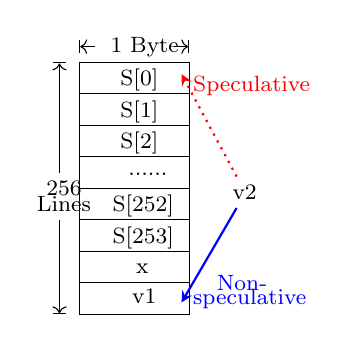
\begin{tikzpicture}[fill=blue!20,font=\footnotesize] 
		\draw[|<-, line width=0.4pt](-0.25, 3.2) -- (-0.25, 1.8);
		\draw[->|, line width=0.4pt](-0.25, 1.2) -- (-0.25, 0);
  	\node[left=4pt, right] at (-0.4, 1.6) {256};
  	\node[left=4pt, right] at (-0.52, 1.4) {Lines};

		\draw (0, 0) rectangle (1.4, 0.4);
  	\node[above=5pt, right] at (0.55, 0.05) {v1};
  	\draw (0, 0.4) rectangle (1.4, 0.8);
		\node[above=5pt, right] at (0.6, 0.4) {x} ;	
  	\draw (0, 0.8) rectangle (1.4, 1.2);
		\node[above=5pt, right] at (0.3, 0.8) {S[253]};
  	\draw (0, 1.2) rectangle (1.4, 1.6);
  	\node[above=5pt, right] at (0.3, 1.2) {S[252]};
  	\draw (0, 1.6) rectangle (1.4, 2.0);
  	\node[above=5pt, right] at (0.5, 1.6) {......};
  	\draw (0, 2.0) rectangle (1.4, 2.4);
  	\node[above=5pt, right] at (0.4, 2.0) {S[2]};
  	\draw(0, 2.4) rectangle (1.4, 2.8);
  	\node[above=5pt, right] at (0.4, 2.4) {S[1]};
  	\draw (0, 2.8) rectangle (1.4, 3.2);
		\node[above=5pt, right] at (0.4, 2.8) {S[0]};

		\draw[|<-, line width=0.4pt](0, 3.4) -- (0.2, 3.4);
		\draw[->|, line width=0.4pt](1.2, 3.4) -- (1.4, 3.4);
  	\node[left=5pt, right] at (0.45, 3.4) {1 Byte};

		\node[left=5pt, right] at (2.0, 1.55) {v2};
    \draw [-stealth,dotted,thick,red](2.0, 1.75)--(1.3, 3.05);
    \draw [-stealth,thick,blue](2.0, 1.35)--(1.3, 0.15);
		\node[left=5pt, right,red] at (1.5, 2.9) {Speculative};
		\node[left=5pt, right,blue] at (1.8, 0.4) {Non-};
		\node[left=5pt, right,blue] at (1.5, 0.2) {speculative};

	  \end{tikzpicture}
\end{minipage}
}
\vspace{-3ex}
\caption{Program $\mathcal{P}$ and its cache mapping.}
\label{fig:motiv}
\end{figure}


\subsection{Leakage-free in Non-speculative Execution}
\label{sec:normal_exec}

Running $\prog$ without speculative execution won't leak any information 
about \texttt{x}. This section analyzes the cache behavior in details. 


There are two program paths in $\prog$ because of the \textit{if-else} 
branch. Let's name the one containing the \textit{if} branch as $p_1$ 
and the other one as $p_2$. The only difference between $p_1$ and $p_2$
is the \emph{store} operation, which writes \texttt{v1} on $p_1$ but 
\texttt{v2} on $p_2$. As analyzed in section~\ref{sec:leak_example}, 
\texttt{v1} would map to the last line of cache $\mathcal{C}$. Similarly, 
without speculative execution, \texttt{v2} also maps to the same line, as 
annotated by the solid arrow in Figure~\ref{fig:2b}. This overlapping 
situation is because usually either $p_1$ or $p_2$ could be taken; 
hence either the \textit{store} to \texttt{v1} or the \textit{store} 
to \texttt{v2} may happen. In both cases, line \#256 is empty before 
the \textit{store} operations. Thereby, \texttt{v1} or \texttt{v2} 
uses this available line.


In view of this fact, we can observe similar cache behaviors on both $p_1$ 
and $p_2$ under non-speculative execution. The first 254 \emph{load} 
operations on array \texttt{S}, the next implicit memory read of \texttt{x},
and the succedent \textit{store} to \texttt{v1} on $p_1$ or to \texttt{v2} 
on $p_2$ all cause cold misses since cache $\mathcal{C}$ is initially empty. 
Likewise, the last memory \emph{load} on \texttt{S[x]} (line 10) must be a 
cache hit on both paths because \texttt{S} and \texttt{x} have already been 
in cache $\mathcal{C}$. In other words, $\prog$'s cache behavior is 
independent of the sensitive input \texttt{x}. As a result, $\prog$ has no 
cache timing leaks under non-speculative execution.


\subsection{New Leak under Speculative Execution}
\label{sec:specu_leak}

In section~\ref{sec:normal_exec}, only one \textit{store} operation can happen 
in non-speculative execution. However, the situation changes, and a new timing 
leak appears when taking speculative execution into account.  


Under speculative execution, the instructions guarded by a branch \emph{br} can 
be scheduled before the execution proceeds into \emph{br} in case CPU predicts 
that \emph{br} is likely to be taken. For example, suppose we first run $\prog$ 
with \texttt{x}$\in$[128,255] several times and flush the cache after each run. 
Afterward, we rerun $\prog$ but setting \texttt{x} to 127. Still, the 
\textit{store} instruction under the \emph{if} branch (line 7) would be executed 
before $\prog$ steers into the \emph{else} branch due to the branch misprediction. 
More importantly, though the CPU performs a rollback to discard the value update 
to \texttt{v1}, \texttt{v1} remains in $\mathcal{C}$ even after the remedy. 


Going until line 9, array \texttt{S} and variable \texttt{x} map from lines \#1 
to \#255 and \texttt{v1} still occupies line \#256. At this point, there is no 
empty line available for \texttt{v2}. Following the LRU policy declared in section
\ref{sec:leak_example}, executing the \textit{store} instruction at line 9 would 
evict the oldest item \texttt{S[0]} from cache $\mathcal{C}$ and map \texttt{v2} 
to the vacated line \#1, as shown by the dotted arrow in Figure~\ref{fig:2b}.


After that, the program execution continues to line 10, reaching the last memory 
\textit{load} of \texttt{S[x]}. Sensitive input \texttt{x} now determines which 
array cell would be visited. And we examine the cache behavior of this \textit{load} 
in terms of two cases \texttt{x=0} and \texttt{x$\neq$0}.


\begin{itemize*}
  \item \texttt{x=0}: $\prog$ reads array cell \texttt{S[0]}. Recall that \texttt{x} 
	is still in cache $\mathcal{C}$, but \texttt{S[0]} is no longer in $\mathcal{C}$ 
	due to the replacement by \texttt{v2}. So this memory \textit{load}	causes a 
	conflicting cache miss.
  \item \texttt{x$\neq$0}: Since the whole array \texttt{S} except \texttt{S[0]}
    is in $\mathcal{C}$, the \textit{load} of \texttt{S[x]} must get a cache hit 
		no matter what value \texttt{x} is.
\end{itemize*}


Only if \texttt{x=0} there appears one more cache miss on path $p_2$. It is a 
unique situation that enables attackers to learn the value of \texttt{x} due to 
a measurable longer execution time. Note that the cold miss from speculatively 
writing \texttt{v1} also causes an internal latency. However, it is un-observable 
to the external users, and we ignore it safely for analysis purposes.


\subsection{What \SpecuSym Should Provide}
\label{sec:app-scenarios}

The example shows that, though a program is carefully crafted to avoid cache 
timing leaks, running it under speculative execution may still exhibit new 
leaks. Since speculative execution is one of the fundamental optimizations 
in modern processors, a systematic analysis that exposes the subtle leaks 
would be of utmost importance. Specifically, we focus on two abilities in 
our new method.


First, \SpecuSym should be able to systematically explore the program state 
space to identify execution paths and speculative flows that may cause leaks. 
E.g., $\mathit{p_2}$ and the speculative execution of the \textit{if} branch. 
Note that speculation of the \textit{else} branch won't cause a similar 
leak along with $\mathit{p_1}$.


Second, \SpecuSym should be able to pinpoint the leak sites by a precise cache 
analysis and generate concrete inputs that witness new cache behavior at the 
identified memory visit sites. E.g., the memory \textit{store} instructions to 
\texttt{v2} and the value \textit{zero} of \texttt{x}.


\section{Preliminaries}
\label{sec:prelim}

This section reviews the preliminary knowledge of symbolic execution, cache timing leak, 
and speculative execution.


%\newpage\clearpage
\subsection{Symbolic Execution}
\label{sec:se}


\begin{algorithm}[hpt]
\caption{Baseline Symbolic Execution.}
\label{alg:baseline}
{\footnotesize
\SetAlgoLined
\setstretch{0.5}
\DontPrintSemicolon
				\nonl \textbf{Initially}: The global state container \textsc{Stack} is empty (\textsc{Stack}$\Leftarrow$$\emptyset$).\\
				\nonl Start \textbf{\SymExec}($\mathit{s_{ini}}$) on an initial state $\mathit{s_{ini}}$ with $\mathit{in:=\{\lambda,t\}}$.\\
\textbf{\SymExec}(SymbolicState $s$)\\
\Begin{
  $\textsc{Stack}$.push($s$);\;

  \uIf{$\mathit{s.e}$ is branch event}{
    \For{$\mathit{c \in s.brs}$ {\bf and} $\mathit{s.pc\wedge c}$ is satisfiable} {
      $\mathit{s.pc\leftarrow s.pc\wedge c}$;\\
      \textbf{\SymExec}($\mathit{SubsequentState}$($\mathit{s}$));~~ \textcolor{dkgreen}{// The $\psi$ event}
    }
  }\uElseIf{$\mathit{s.e}$ is memory access event}{
    \textbf{\SymExec}($\mathit{SubsequentState}$($\mathit{s}$));~~ \textcolor{dkgreen}{~~~~~~~// The $\chi$ event}
  }\uElseIf{$\mathit{s.e}$ is other interpretable event}{
    \textbf{\SymExec}($\mathit{SubsequentState}$($\mathit{s}$));~~~~~~~~~ \textcolor{dkgreen}{// The $\varphi$ event}
  }\Else{
    Terminate state $s$;\;
  }
  $\textsc{Stack}$.pop();\;
}

\BlankLine

\textit{SubsequentState} (SymbolicState \textit{s})\;
\Begin{
  $\mathit{s'} \leftarrow$ symbolically execute $\mathit{e.inst}$ in $\mathit{s}$;\;
  $\mathit{s'.e} \leftarrow$ next available event;\;
  \textbf{return} $s'$;
}
}
\end{algorithm}



Symbolic execution, as a systematic program testing and analysis technique, 
was first introduced in the 1970s~\cite{King76,Clarke76}. In this work, we 
assume that a program $\prog$ consists of a finite set of instructions, and 
$\prog$ defines execution semantics in program paths. Let \textit{inst} be 
an instruction, then interpreting an event $e$:=$(l_b\succ inst\succ l_a)$ 
in symbolic execution stands for the execution of \textit{inst} where $l_b$ 
and $l_a$ denote the locations before and after $inst$, respectively. A 
program execution explores a sequence of events along the program path. 
Close to~\cite{GuoKWYG15,GuoWW18}, we abstract a symbolic event $e$ into 
three categories in terms of the type of \textit{inst} that $e$ contains.


\begin{itemize*}
  \item $\psi$-event, which presents a branch decision. It models the 
    \textit{then} branch by \textcode{assume$(c)$} and the \textit{else} 
    branch by \textcode{assume$(\neg c)$}, respectively. Term $\textit{c}$ 
    is the representative of a conditional predicate expressed in symbolic 
    expression. 

  \item $\chi$-event, which corresponds to a memory \textit{read} instruction 
    of the form $\textit{var}=\textit{load~addr}$, or a memory \textit{write} 
    instruction like $\textit{store~addr, expr}$ where \textit{addr} is the 
    memory address, and \textit{expr} is a symbolic expression.

  \item $\varphi$-event, which represents other types of instructions in the 
    form $\textit{var}:=\textit{expr}$. Here \textit{var} is a variable, and 
    \textit{expr} is a symbolic expression computed from preceding operations 
    like arithmetic calculation, bit manipulation, etc.
\end{itemize*}


Although symbolic executors always support a rich set of instructions, we use 
the above event types to abstract away the internal implementation details like 
memory allocation, function return, and et.al., to center on the high-level 
flow of symbolic execution. Algorithm~\ref{alg:baseline} presents the baseline 
symbolic execution of a program with sensitive input. Unlike prior works
\cite{GuoKWYG15,GuoWW18}, both global and local memory accesses are uniformly
handled. The data input, $\mathit{in}:=\{\lambda,t\}$, determines a program 
execution path consisting of ordered events $\{e_1,\ldots,e_n\}$ where 
$\mathit{\lambda}$ is the sensitive input, e.g., privacy data or cipher keys, 
and $\mathit{t}$ is the insensitive input.


The \textsc{Stack} is a global container for storing symbolic states during 
dynamic exploration. A symbolic state $\mathit{s}$ exhibits the frontier of 
a path execution. We define $\mathit{s}$ as a tuple $\langle \pcon, \mathit{e},
\mathit{brs}, \Omega \rangle$. $\pcon$ denotes the path condition that leads 
to $\mathit{s}$ where $\mathit{e}$ is the event to execute at $\mathit{s}$. 
$\mathit{brs}$ contains the set of branch predicates if $\mathit{e}$ is a 
$\psi$ event. And $\Omega$ is the symbolic memory which maintains the mappings 
from the program variables to their memory values at $\mathit{s}$.


Initially, the state container \textsc{Stack} is empty, and we start the main 
procedure \SymExec with the initial state $\mathit{s_{ini}}$ on input $\mathit{in}$.
During the recursive execution, \SymExec may split a branch (lines 4-8), perform 
a memory operation (lines 9-10), conduct an internal computation (lines 11-12), 
or terminate a state (line 14), depending on the type of the event to execute.


Note that at the entry of each recursion, \SymExec takes a new symbolic state 
as the input, which is obtained from invoking a secondary procedure 
\textit{SubsequentState}. This procedure accepts the current state 
\textit{s} as the input and outputs a new state $s'$ by symbolically executing 
the \textit{inst} in \textit{s.e}. For brevity, we omit the details of the 
instruction interpretation, which can be found in~\cite{CadarDE08,PasareanuR10}.



\subsection{Cache Timing Leak}
\label{sec:leak}

Memory operations are prone to timing leaks because of the outstanding accessing 
latency between the cache and the main memory. For example, reading data from the 
cache may cost 1-3 processor cycles, whereas loading data from memory could spend 
hundreds of cycles. In this section, we first establish the threat model and then 
formalize the leak definition based on the threat model.


\subsubsection{The Threat Model}
\label{sec:threat}

As exhibited in Section~\ref{sec:specu_leak}, sensitive data involved in memory 
access may get leaked from the timing traffic of a memory write. To capture such 
kind of subtle leak in our analysis, we assume the attackers can perform strong 
external threats. 


First, we assume the attackers share the same processor with the victim process. 
Hence they can learn the shared cache states by probe methods. Second, they are 
allowed to request the execution of the victim process. Third, they can observe 
the latency of the interested memory visits in the victim process. Our threat 
model is close to those used in practical attacks like
\cite{OsvikST06,YaromF14,DisselkoenKPT17}, where the attackers can deduce the 
cache block states by measuring the timing traffic of either the victim or the 
attacker process. Moreover, this model also appears in leak detection techniques 
like~\cite{WangWLZW17,DoychevK17,WichelmannMES18,BrotzmanLZTK2018}. Therefore, 
we believe it is a reasonable model for analysis purposes.
%without strong acquisition of system priviledges.


\subsubsection{The Leak Definition}

Formally, we abstract a sensitive data related program $\prog$ to be a function 
$\mathit{F_{\prog}(in)\Rightarrow out}$. $\mathit{F_{\prog}}$ processes the data 
input $\mathit{in}:=\{\lambda,t\}$ (cf. section~\ref{sec:se}) and returns the 
output $\mathit{out}$. E.g., assuming $\prog$ is an encryption process, $\lambda$ 
is the private key, and $t$ is the content to encrypt; then, $out$ is the ciphertext. 
Let $T(F_{\prog}(in))$ denotes the execution time of $\prog$ with input $\mathit{in}$ 
under non-speculative execution. Different inputs may explore various program paths. 
However, since we aim at timing leaks introduced by speculative execution, here we 
assume the time of those non-speculative program executions remain similar or the 
same, no matter what the sensitive inputs are, which is, 
%
\begin{multline} 
  \label{lb:no_leak_event}
  ~~~~~\mathit{\forall t,\lambda,\lambda'~.~T(F_{\prog}(\lambda,t)) \simeq 
  T(F_{\prog}(\lambda',t))}~~~~
\end{multline} 
%
Symbols $\lambda$ and $\lambda'$ denote any two sensitive inputs, and $t$ is still 
the public input. Nevertheless, since in practice, attackers may gain information 
by observing several memory visits or cache lines, we restrict the leak granularity 
at the memory operation level regarding our threat model. Specifically, let $\mathit{e}$ 
be a memory event on executing $\prog$ and the time of interpreting $\mathit{e}$ with 
and without speculative execution be 
$\mathit{T_{s}(\prog_e(in))}$ and $\mathit{T(\prog_e(in))}$, we assume:
%
\begin{multline} 
  \label{lb:no_leak_event}
  ~~~~~\mathit{\forall t,\lambda,\lambda'~.~T(\prog_e(\lambda,t)) \simeq 
  T(\prog_e(\lambda',t))}~~~~
\end{multline} 
%
Then the existence of a new cache timing leak under speculative execution can be 
checked by the following formula: 
%
\begin{multline}
\label{lb:specu_leak}
\mathit{\exists t,\lambda,\lambda'~.~
	\big(
			\lambda \neq \lambda' \wedge T_{s}({\prog_e}(\lambda,t)) 
			\neq T_{s}({\prog_e}(\lambda',t))}
	\big)
	\vee 
	\\  
	T({\prog_e}(\lambda,t)) \neq T_{s}({\prog_e}(\lambda',t)) ~~~
\end{multline}
%
where a leak appears if (1) two different sensitive inputs can cause significant 
timing differences in executing $\mathit{e}$ under speculative execution, or (2) 
two sensitive inputs can cause significant timing difference in executing $\mathit{e}$ 
with and without speculative execution. In other words, $\prog$ leaks due to 
speculative execution if any pair of $\lambda$ and $\lambda'$ exists. Furthermore, 
we transform formula (\ref{lb:specu_leak}) into a dedicated leak constraint and 
simplify the constraint to a more concise form in section~\ref{sec:specuSE}. Also, 
as public input plays a minor role in modeling cache timing leaks~\cite{WangBLWZW19}, 
we set insensitive input $t$ to a fixed value to reduce the reasoning cost of formula
(\ref{lb:specu_leak}). 

\ignore{
Also, we assume $\prog$ has the same set of instructions on each program path and 
speculative execution only changes the cache state. 
}



\subsection{Speculative Execution}
\label{sec:specu}

The instruction pipeline~\cite{RamamoorthyL77} in processor allows overlapped 
executions of proper instructions where each instruction execution has a series 
of stages. This instruction-level parallelism benefits hardware utilization since 
an instruction can start its stage prior to the time its preceding instructions 
have finished all their stages. However, a pipe-lined processor may get stalled 
once the program control flow needs to divert but the destination remains unknown 
(e.g., at a conditional branch). Accordingly, the pipeline has to await until 
the flow decision is computed.


To alleviate the cost of this control hazard, modern processors leverage 
\textit{branch prediction}~\cite{Mittal19} and \textit{speculative execution}
\cite{kimuraKT1996} to reduce the delay that could incur w.r.t conditional branch 
instructions. Generally, they predict the execution flow upon the history of 
recently executed branches, and schedule instructions under predicted branches
ahead of jumping into these branches. 
Specifically, on approaching a control hazard the processors first predict which 
branch to be taken. Then, they execute the selected branch and maintain the 
temporary path state in a dedicated buffer. Finally, they commit the buffered 
state to continue the program flow if the prediction is correct. Otherwise, upon 
an incorrect prediction, they have to discard the temporary state to revert the 
effects of the executed instructions hence avoiding functional errors. 


This rollback mechanism, unfortunately, withdraws no affected cache state, which 
raises security risks. As shown in Figure~\ref{fig:2b}, variable \texttt{v2} 
may map to cache line \#256 due to speculative execution of the \textit{else} 
branch. Moreover, this affect is not eliminated when control flow is redirected
to the \textit{if} branch because of the misprediction. As a result, sensitive
data \texttt{x} leaks over the altered cache state. 
Abstracting away the hardware details, we can precisely model the behavior of 
speculative execution in symbolic execution as a three-step process and evaluate
its side effects to the cache state with a constraint-solving based approach. 


\textbf{Misprediction Modeling.}
As aforementioned, on reaching a control hazard the processors predict the hazard
result to select a branch. Despite the experience-based hardware realization, we 
can model this behavior by auxiliary symbolic state. To be specific, before 
diverging the control flow into the \textit{if} branch, our symbolic executor 
would decide to duplicate a new state from the current symbolic state and schedule
it immediately into the \textit{else} direction, which represents the speculative 
execution of the \textit{else} branch. 

%Similarly, we can perform the 
%symmetrical simulation for the \textit{if} branch on demand.

\ignore{
Note that we only model speculative execution at branches where both \textit{if} 
and \textit{else} decisions are feasible in terms of the branch conditions. The 
assumption considers the situation where the hazard is dependent on the computation 
over input and cannot be inferred as a \textit{true} or a \textit{false} value in 
advance. In contrast, if the condition is determined to be \textit{true} or 
\textit{false} at the branch point, e.g., the \textit{while} loop head in Figure
\ref{fig:fig2-a}, then the branch decision is deterministic.
}

\ignore{
However, different program inputs might go through various program paths to reach 
a same branch point but trigger divergent decisions. Thus, in practice speculative 
executions at these points do exist and our method complies with the fact.
}


\textbf{Speculative State Execution.}
Each duplicated state in \textit{misprediction modeling} has the same 
memory snapshot to its parent symbolic state. For clarity, we use 
\textit{speculative} state to name the new state. A \textit{speculative} 
state will be prioritized to the head of the state queue in the symbolic 
executor, and executes uninterruptedly until it meets a predefined threshold, 
such as the maximum instruction number in the Reorder Buffer (ROB), the 
pipeline stage number, the branch depth, and etc. Owing to the 
\textit{copy-on-write} schema in modern symbolic executors
\cite{CadarDE08,CiorteaZBCC09}, the \textit{speculative} state runs 
independently from their parent symbolic state. The memory updates in a 
\textit{speculative} state won't taint its parent state who waits at the 
state-forking point for the \textit{speculative} state returns. For the 
sake of cache analysis, we model the runtime cache state in each symbolic 
state. A \textit{speculative} state inherits this data from its parent 
and keeps updating the cache during its execution.


\textbf{Rollback and Cache Merging.}
Once a \textit{speculative} state reaches the threshold, it has to 
stop and quit the state queue. Right before its termination, it 
notifies the awaiting parent state the finish of the current speculative execution, 
as well as transfers the cache status back to the parent. On 
receiving the notification, the parent symbolic state merges the 
speculated cache into its own cache to form the latest cache state. After 
that, the parent aborts waiting and resumes the normal execution.
This step models the processor rollback mechanism in high fidelity
and retains the changed cache state from speculative execution. 
Terminating the \textit{speculative} state eliminates any further 
affects and the latest cache status has already been absorbed 
into the parent state. This approach is natural to symbolic execution, 
while the existing simulation~\cite{OleksenkoTSF19} method requires 
sophisticated instrumentations and specific instructions to enforce 
CPU behaviors. More technical details will be presented in section
\ref{sec:spec_modeling}.

\ignore{
Our modeling approach is sound and elegant. Focusing on the worst 
case predication, we avoid missing any speculated branch that may 
cause leaks. 
}


%\newpage\clearpage
\section{Speculative Symbolic Execution}
\label{sec:specuSE}

In this section we present the core algorithm of \SpecuSym, and explain 
the technical contributions listed in Figure~\ref{fig:overall_flow}. 
Algorithm~\ref{alg:specusym} shows the main algorithm of \SpecuSym, 
where the major changes from the baseline algorithm are at the state 
checkpoint (lines 3-5), the branch point (line 9), and the memory 
access point (lines 14-15). We highlight these changes in blue. 


\begin{algorithm}[t]
\caption{Symbolic Execution in \SpecuSym.}
\label{alg:specusym}
{\footnotesize
\SetAlgoLined
\setstretch{0.5}
\DontPrintSemicolon
\nonl \textbf{Initially}: The global state container \textsc{Stack} is empty (\textsc{Stack}$\Leftarrow$$\emptyset$).;\\
\nonl Start \textbf{\SpecuSym}($\mathit{s_{ini}}$) on an initial symbolic state $\mathit{s_{ini}}$ with $\mathit{in:=\{\lambda,t\}}$.\\
\textbf{\SpecuSym}(SymbolicState $s$)\\
\Begin{
				\If{\textcolor{blue}{$\mathit{s}$ is a speculative state} {\bf{and}} \textcolor{blue}{$\mathit{s}$ reaches the threshold}}{
								\textcolor{blue}{\textbf{return};}\;
					}
				$\textsc{Stack}$.push($s$);\;
        \uIf{$\mathit{s.e}$ is branch event}{
          \For{$\mathit{c \in s.brs}$ {\bf and} $\mathit{s.pc\wedge c}$ is satisfiable} {
            \textcolor{blue}{$\mathit{SpeculativeExplore}$($s$, $c$);}~~~~~~~~~~\textcolor{dkgreen}{// Enter speculative modeling}\;
            ......~~~~~~~~~~~~~~~~~~~~~~~~~~~~~~~~~~~~~~~~~~~~~\textcolor{dkgreen}{// Resume normal execution}\;

          }
        } 
        \uElseIf{$\mathit{s.e}$ is memory access event}{
          \textbf{\SpecuSym}($\mathit{SubsequentState}$($\mathit{s}$));\;	
          \textcolor{blue}{$\mathit{AnalyzeCache}$($s$);}\;
          \textcolor{blue}{$\mathit{s}.\varpi\leftarrow $ update cache state by interpreting $\mathit{s.e}$;}\;
        }
        ......\;
}
~~~\\
$\mathit{SpeculativeExplore}$(SymbolicState $s$, Predicate $c$)\;
\Begin{
  \If{$\mathit{c}$ relies on a memory visit}{
    $\mathit{s' \leftarrow }$ duplicate state $\mathit{s}$;~~~~~~~~~~~~~~~~~~~~~~~~~~~~~\textcolor{dkgreen}{// Fork speculative state}\;
    $\mathit{s' \leftarrow redirect~s'~to~the~\neg c~control~flow}$;~~\textcolor{dkgreen}{// Redirect execution flow}\;
    \textbf{\SpecuSym}($\mathit{SubsequentState}$($\mathit{s'}$));\;
    $\mathit{s}.\varpi \leftarrow \mathit{s'}.\varpi$;\;%\mathit{s}.\Xi \diamond 	
    Terminate $\mathit{s'}$;\;
  }
}
~~~\\
$\mathit{AnalyzeCache}$(SymbolicState $s$)\;
\Begin{
    \If{$\mathit{s}$ is a regular symbolic state {\bf{and}} s.e relates to secret input}{
    $\xi\leftarrow$ build the leak constraint for $\mathit{s.e}$;\;
    \If{$\mathit{s.pc}\wedge\xi~\mathit{is~satisfiable}$}{
      Generate witness;\;
    }
  }
}
}
\end{algorithm}



\subsection{Speculative Modeling}
\label{sec:spec_modeling}

%In this section we show how \SpecuSym models branch mispredictions and
%speculative execution by introducing auxiliary symbolic states and 
%orchestrating them in proper orders.

On entering the \SpecuSym procedure, our new algorithm first checks 
if the current state $s$ is a \textit{speculative~state}, and whether 
$s$ has reached the predefined threshold (line 3). If both conditions
are met, \SpecuSym stops the recursive symbolic execution on $s$ and 
returns immediately (line 4). A state becomes a \textit{speculative 
state} if it is duplicated from a regular symbolic state (line 22) by
invoking \textit{SpeculativeExplore} at a branch event (line 9). 

%At the high level, subroutine $\mathit{SpeculativeExplore}$ models 
%branch mispredictions with extra symbolic states, and updates the
%cache on exploring these auxiliary states.

Lines 19-28 in Algorithm~\ref{alg:specusym} present the modeling procedure 
\textit{SpeculativeExplore}. Generally, at a conditional branch (line 8), 
we call \textit{SpeculativeExplore} (line 8) to start the speculative probe. 
That is, if the branch predicate relies on a memory access (line 21), e.g.,
using a static variable for the first time, we then duplicate a new state 
$s'$ from state \textit{s} (line 22) with a negated execution flow (line 23). 
This assumption is based on the observation that the memory visiting latency 
at a branch point may create a time window for speculative execution to load 
data into cache before the rollback. Otherwise, despite a branch misprediction, 
the CPU only spends several cycles on restoring before speculative execution 
takes effect on cache.


%Similarly, we also fork another state for 
%modeling the symmetrical misprediction. 

The new state ${s'}$ becomes a \textit{speculative state} afterwards, since 
it is about to mimic the speculative execution of the mis-predicted branch 
before resuming $s$. After state duplication, we let \SpecuSym execute $s'$ 
(line 24) and evaluate the effects of the memory visits in $s'$ on the cache 
(line 15). Details of the evaluation will be presented in section
\ref{sec:modeling}. Once the recursive exploration of $s'$ finishes, we use 
the accumulated cache state in $s'$ to update that of $s$ (line 25) and 
terminate $s'$ (line 26). The termination ends the lifetime of state $s'$. 
It also assures that the execution in $s'$ only attributes to the cache 
state changes but never affects the memory state of its parent state.

%\HB{: hard to understand this sentence: "is only attributes, but never affects"}


Next, when $\mathit{SpeculativeExplore}$ returns, we resume the normal 
execution on $s$ (line 10), with an updated cache state. In this way, 
we construct the speculative scenario and retain the latest cache. Our 
approach leverages the stateful feature of symbolic execution. It not only 
models the speculative behavior but also seamlessly stitches the cache
state with controllable flexibility. 


Figure~\ref{fig:specu_modeling} shows the speculative modeling of 
the example $\prog$ from Figure~\ref{fig:motiv}. Figure~\ref{fig:fig3-a} 
gives the control flow graph of $\prog$ on which we annotate the memory 
access related variables. For example, {S[0]} means the first array read in the 
$\mathit{while}$ loop and \texttt{v1} means the memory \emph{write} in 
the $\mathit{if}$ branch. The blue arrow line denotes the flow of the 
symbolic state $s$ which takes the $\mathit{if}$ branch in regular 
symbolic execution. 


Then, in Figure~\ref{fig:fig3-a}, on reaching the branch we duplicate a 
\textit{speculative} state $s'$ from $s$, and enforce a bounded execution
(e.g., one memory access) into the \textit{else} branch of $s'$, as shown 
by the red dashed line. Once $s'$ meets the threshold, we stop the 
execution and turn back to its birth point where state $s$ is awaiting 
the finish of $s'$. Also, we integrate the cache state of $s'$ (cf. 
Figure~\ref{fig:fig3-b}) into $s$ and terminate $s'$ to resume $s$. Right 
now, the whole cache has been filled since the memory write in $s'$ mapped 
\texttt{v2} into the line \#256 . 


Subsequently, the memory \emph{store} to \texttt{v1} in state $s$ has to 
replace \texttt{S[0]} following the LRU policy, as shown in Figure
\ref{fig:fig3-b}. Also, the last memory \emph{load} to \texttt{S[x]} might 
result in a cache miss or a cache hit, depending on the value of \texttt{x}, 
which is consistent with the situation in section~\ref{sec:specu_leak}. 
Hence, our proposed method succeeds in modeling speculative execution 
and conforms to the three-step process designed in section~\ref{sec:specu}. 
Note that Figure~\ref{fig:fig3-a} only shows the modeling of the \emph{else} 
branch while \SpecuSym considers both branches and misses no potential cases. 

%Also, we can use different bounds of the speculative state for more practical 
%cache analysis.


\ignore{
In Figure~\ref{fig:fig3-a}, the speculative state $s'$ inherits the cache 
state from $s$, maps \texttt{v2} into a cache line, and merges back the updated 
cache state to state $s$ before its termination, as formally stated in Algorithm
\ref{alg:specusym} (lines 24-26). 
}


In this example, updating the cache state is straightforward -- by checking 
the in-cache addresses to find an available cache line on a cache miss, or 
retain the current cache items in case of a hit. For the undecided address, 
i.e., \texttt{S[x]}, we can try 255 possible cache mappings to test the 
difference. However, it is impractical to eagerly enumerate all potentials since it can 
cause unbearable overhead. Abstract interpretation based analysis~\cite{WuW19} 
approximates concrete possibilities whereas this approach is impractical in 
symbolic execution. Also, many mappings are indeed redundant w.r.t leak 
exposure, e.g., only 1 mapping reveals leak in the motivating example. 


Instead, \SpecuSym models all possible branch mispredictions along with  an execution 
path to maintain a \textit{stitched} trace of memory events as the alternative 
of the cache state. Then it builds the leak constraint by analyzing the trace, 
and lazily searches for solutions. We detail this trace-based analysis in section
\ref{sec:modeling} and section~\ref{sec:analysis}. 


\begin{figure}%[htb]
\subfigure[Stitched executions of $s$ and $s'$]{
\label{fig:fig3-a}
\begin{minipage}{0.4\linewidth}
	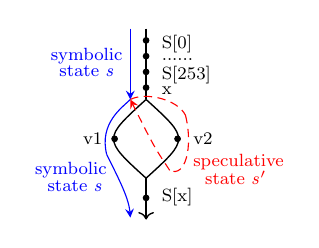
\begin{tikzpicture}[fill=blue!20,font=\footnotesize] 

		\draw[->, line width=0.5pt, black](0, 0.8) -- (0, 0.275);
		\draw[line width=0.5pt, black](0, 1.8)..controls (-0.55,1.3) .. (0, 0.8);
		\draw[line width=0.5pt, black](0, 1.8)..controls (0.55,1.3) .. (0, 0.8);
		\draw[line width=0.5pt, black](0, 2.7) -- (0, 1.8);

		\filldraw [black] (0, 2.55) circle (1pt);
		\filldraw [black] (0, 2.35) circle (1pt);
		\filldraw [black] (0, 2.15) circle (1pt);
		\filldraw [black] (0, 1.95) circle (1pt);
		\filldraw [black] (-0.4, 1.3) circle (1pt);
		\filldraw [black] (0.4, 1.3) circle (1pt);
		\filldraw [black] (0, 0.55) circle (1pt);

    \node[above=3pt, right, scale=.8] at (0.1, 2.4) {S[0]};
  	\node[above=3pt, right, scale=.8] at (0.1, 2.2) {......};
		\node[above=3pt, right, scale=.8] at (0.1, 2.0) {S[253]};
		\node[above=3pt, right, scale=.8] at (0.1, 1.8) {x};
		\node[above=3pt, right, scale=.8] at (-0.9, 1.2) {v1};
    \node[above=3pt, right, scale=.8] at (0.5, 1.2) {v2};
    \node[above=3pt, right, scale=.8] at (0.1, 0.45) {S[x]};

    \draw [-stealth,thin,blue](-0.2, 2.7)--(-0.2, 1.8);
		\draw [thin,blue](-0.2, 1.8)..controls (-0.3, 1.7) and (-0.6, 1.5) .. (-0.5, 1.1);
		\draw [-stealth,thin,blue](-0.5, 1.1)..controls (-0.3, 0.7) and (-0.2, 0.5) .. (-0.2, 0.3);

		\node[above=3pt, left, scale=.8, blue] at (-0.2, 2.25) {symbolic};
		\node[above=3pt, left, scale=.8, blue] at (-0.3, 2.05) {state $\mathit{s}$};
		\node[above=3pt, left, scale=.8, blue] at (-0.4, 0.8) {symbolic};
		\node[above=3pt, left, scale=.8, blue] at (-0.45, 0.6) {state $\mathit{s}$};

		\draw [densely dashed, thin,red](-0.2, 1.8)..controls (0, 1.9) and (0.4, 1.8) .. (0.5, 1.6);
		\draw [densely dashed, thin,red](0.5, 1.6)..controls (0.6, 1.2) and (0.5, 0.8) .. (0.3, 0.9);
		\draw [-stealth, densely dashed, thin,red](0.3, 0.9)..controls (0.1, 1.2) .. (-0.2, 1.8);

		\node[above=3pt, right, scale=.8, red] at (0.5, 0.9) {speculative};
		\node[above=3pt, right, scale=.8, red] at (0.65, 0.7) {state $\mathit{s'}$};

	  \end{tikzpicture}
\end{minipage}
}
\subfigure[The cache state from $s'$]{
\label{fig:fig3-b}
\begin{minipage}{0.3\linewidth}
	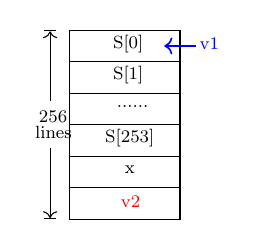
\begin{tikzpicture}[fill=blue!20,font=\footnotesize] 
		\draw[->|, line width=0.4pt](-0.25, 1.7) -- (-0.25, 2.6);
		\draw[->|, line width=0.4pt](-0.25, 1.1) -- (-0.25, 0.2);

  	\node[left=4pt, right, scale=.8] at (-0.35, 1.5) {256};
  	\node[left=4pt, right, scale=.8] at (-0.4, 1.3) {lines};

  	\draw (0, 0.2) rectangle (1.4, 0.6);
		\node[above=5pt, right, scale=.8, red] at (0.55, 0.25) {v2} ;	
  	\draw (0, 0.6) rectangle (1.4, 1.0);
		\node[above=5pt, right, scale=.8] at (0.6, 0.65) {x};
  	\draw (0, 1.0) rectangle (1.4, 1.4);
  	\node[above=5pt, right, scale=.8] at (0.35, 1.05) {S[253]};
  	\draw (0, 1.4) rectangle (1.4, 1.8);
  	\node[above=5pt, right, scale=.8] at (0.5, 1.45) {......};
  	\draw (0, 1.8) rectangle (1.4, 2.2);
  	\node[above=5pt, right, scale=.8] at (0.45, 1.85) {S[1]};
  	\draw(0, 2.2) rectangle (1.4, 2.6);
		\node[above=5pt, right, scale=.8] at (0.45, 2.25) {S[0]};
		\node[above=5pt, right, scale=.8, blue] at (1.55, 2.25) {v1};

		\draw[<-, line width=0.6pt, blue] (1.2, 2.4) -- (1.6, 2.4) ;

	\end{tikzpicture}
\vspace{.3ex}
\end{minipage}
}
\vspace{-3ex}
\caption{The speculative execution modeling of $\prog$.}
\vspace{-3ex}
\label{fig:specu_modeling}
\end{figure}



\subsection{Cache State Modeling}
\label{sec:modeling}

%The cache state during a program execution refers to the status of the 
%cache lines after executing every memory-related instruction, e.g., the 
%cache snapshot shown in Figure~\ref{fig:fig3-b}.

This section explains how \SpecuSym models the cache state. Since each explored 
path in symbolic execution represents a unique program run, we thereby extend 
the definition of a symbolic state $s$ (cf. section~\ref{sec:se}) to be a new 
tuple $\langle \pcon, \mathit{e}, \mathit{brs}, \Omega, \varpi \rangle$. The 
newly introduced symbol $\varpi$ denotes the cache state on exploring $s$.
Based on this design, we establish notions as following:
%
%
\begin{itemize*}
  \item [$-$]A program state in \SpecuSym is either a normal \textit{symbolic} 
    state or a \textit{speculative} state, where from the former can the latter 
    be duplicated, but not vice versa. 
  \item [$-$]A stitched memory event trace, denoted as $\mathit{M}=\mathit{\{m_0,...,m_n\}}$, 
    consists of executed memory events in the execution order.
  \item [$-$]Each memory event $\mathit{m_i}$ in $\mathit{M}$, where index 
    $i\in [0,n]$, can be from a \textit{symbolic} state or a \textit{speculative}state.
  \item [$-$]The cache state $\varpi$ of a program state, is alternatively
    represented by $\mathit{M}$ and the related computation.
\end{itemize*}
%
%
\ignore{
On modeling the cache state, exsiting tools such as CaSym~\cite{BrotzmanLZTK2018} 
maintains and updates cache mappings during symbolic execution; others like 
Chalice~\cite{ChattopadhyayBRZ17} and \textsc{SymSC}~\cite{GuoWW18} uses 
offline constraint solving to to reason about the cache behaviors of memory 
accesses upon concrete cache models. To better coordinate the speculative 
modeling component, \SpecuSym adopts an on-the-fly analysis.
}

To be specific, after executing a memory event $m_i$ in a \textit{symbolic} state, 
we analyze if $\mathit{m_i}$ may lead to timing leak under two scenarios, namely 
new \textit{divergent} behavior and new \textit{opposite} behavior. To formally 
explain these scenarios, we define the following notions.

%
\begin{itemize}
  \item [$-$]$\mathit{\mu_{in}(m_i)}$ denotes the condition satisfying which 
    $\mathit{m_i}$ can trigger a cache hit under speculative execution with 
    input $\mathit{in}$. 
  \item [$-$]$\mathit{a_i}$ denotes the accessed memory address in $\mathit{m_i}$.
  \item [$-$]$\mathit{cs(a_i)}$ denotes the cache set that $\mathit{a_i}$ 
    maps to.
  \item [$-$]$\mathit{tag(a_i)}$ denotes the unique $\mathit{tag}$ of $\mathit{a_i}$.
  \item [$-$]{N} denotes the cache associativity (i.e., N-way set associative 
    cache, where N$\in$[1, the total number of cache lines]). 
\end{itemize}
%


\subsubsection{New Opposite Behavior}
\label{sec:new_opp}
It means executing $\mathit{m_i}$ under speculative execution causes a 
always-hit then the cache behavior in non-speculative execution must be
a always-miss, and vice versa. Recall that we only target new leaks from 
speculative execution and this scenario depicts the exactly opposite leak
behavior. To establish its definition, we introduce following new notions: 

%
\begin{itemize}
  \item [$-$]$\mathit{\eta_{in}(m_i)}$ denotes the condition satisfying which 
    $\mathit{m_i}$ \textit{always} triggers a cache hit under speculative 
	execution.
  \item [$-$]$\mathit{\eta^\prime_{in}(m_i)}$ denotes the condition satisfying which 
    $\mathit{m_i}$ \textit{always} triggers a cache hit under non-speculative
	execution.
  \item [$-$]Boolean variable $\mathit{org(m_i)}$ shows the origin of $\mathit{m_i}$, 
    where 0 means $\mathit{m_i}$ is from a \textit{symbolic} state and 1 means 
    $\mathit{m_i}$ is from a \textit{speculative} state.
\end{itemize}
%

Then we formalize $\mathit{\eta_{in}(m_i)}$ and $\mathit{\eta^\prime_{in}(m_i)}$ as follows. 
%
\begin{multline}
  \label{eqn:hc1}
    \mathit{\eta_{in}(m_i)}~:=~~ 
     \underbrace{ 
      \exists\mathit{j}\in[\mathit{0,i})|
      \wedge 
      \mathit{a_j}=\mathit{a_i} 
    ~\wedge~
      {\forall}x\in\left(j,i\right)\big|\mathit{a_x}\ne\mathit{a_i}
    }_{{\circled{1}}\mathit{~Find~the~nearest~identical~address~a_j}}
		~~~\wedge 
		\\
    ~~~~\sum_{{\scriptscriptstyle \mathit{y=j}+1}}^{{\scriptscriptstyle \mathit{i-}1}} 
    \underbrace{
      \mathit{cs(a_j)}=\mathit{cs(a_y)} 
      \wedge
      \nexists\mathit{z}\in(\mathit{j,y})|\mathit{tag(a_z)}=\mathit{tag(a_y)}
    }_{{\circled{2}}\mathit{~Count~the~unique~a_y~who~and~a_i~map~to~the~same~set}}
    <N
\end{multline}
\vspace{.2ex}
\begin{multline}
  \label{eqn:hc2}
    \mathit{\eta^\prime_{in}(m_i)}:=\mathit{\eta_{in}(m_i)}\wedge
    \underbrace{
      \mathit{org(a_j)}\ne1 
      \wedge
      \mathit{org(a_x)\ne}1 
      \wedge
      \mathit{org(a_y)\ne}1 
    }_{{\circled{3}}\mathit{~Filter~events~from~speculative~execution}}
\end{multline}
%
%
Given a $\mathit{m_i}$, we first search $\mathit{M}$ for an identical 
address $\mathit{a_j}$ ($\mathit{a_i}$=$\mathit{a_j}$) who was 
visited before $\mathit{m_i}$. Also, $\mathit{a_j}$ has to be the nearest 
candidate that no other addresses between $\mathit{a_j}$ and $\mathit{a_i}$ 
are qualified (cf. \circled{1}). Second, we count the unique addresses that 
map to the same cache set to $\mathit{m_i}$ and assure the sum is less than 
the set associativity (cf. \circled{2}). Note that $\mathit{\eta_{in}(m_i)}$ 
is close to but not equivalent to $\mathit{\mu_{in}(m_i)}$. E.g., for 
\texttt{S[x]} \textit{read} in Figure~\ref{fig:fig3-a}, $\mathit{\mu_{in}(m_i)}$ 
can be satisfied but $\mathit{\eta_{in}(m_i)}$ cannot.

Based on $\mathit{\eta_{in}(m_i)}$ we define $\mathit{\eta^\prime_{in}(m_i)}$
who has an extra constraint (cf. \circled{3}) over $\mathit{\eta_{in}(m_i)}$. 
The new constraint ensures that all involved memory events must be from 
\textit{symbolic} states hence filtering the influences of memory events 
from \textit{speculative} states.

\subsubsection{New Divergent Behavior}
\label{sec:new_div}
It means executing $\mathit{m_i}$ under speculative execution with two inputs 
$\mathit{in}$ and $\mathit{in'}$ can cause a miss and a hit, respectively. To
analyze this behavior, we build $\mathit{\mu(m_i)}$ which returns the cache hit
condition of $\mathit{m_i}$ in trace $\mathit{M}$ as follows:
%
%
\begin{multline}
  \label{eqn:hc}
    \mathit{\mu_{in}(m_i)}:=
    \bigvee_{{\scriptscriptstyle 0{\leq}j<i}}
    \Big(
    \underbrace{
      \mathit{tag(a_j)}=\mathit{tag(a_i)} 
			\wedge 
      \mathit{cs(a_j)}=\mathit{cs(a_i)} 
    }_{{\circled{4}}\mathit{~Identify~the~potential~a_j}}
    ~~~~~~\wedge 
		~~\\
    \underbrace{
      {\forall}x\in\left(j,i\right)\big |\mathit{tag(a_x)}\ne\mathit{tag(a_i)}
      \vee 
      \mathit{cs}(a_x)\ne\mathit{cs}(a_i)
    }_{{\circled{5}}\mathit{~Find~the~nearest~a_j}}
		~~~\wedge 
		\\
    \sum_{{\scriptscriptstyle \mathit{y=j}+1}}^{{\scriptscriptstyle \mathit{i-}1}} 
    %\Big(
    \underbrace{
      \mathit{cs(a_j)}=\mathit{cs(a_y)} 
      \wedge
      \nexists\mathit{z}\in(\mathit{j,y})|\mathit{tag(a_z)}=\mathit{tag(a_y)}
    }_{{\circled{6}}\mathit{~Count~the~unique~a_y~who~and~a_i~map~to~the~same~set}}
    <N 
    \Big)
\end{multline}
\vspace{.8ex}
%
%

Given a $\mathit{m_i}$, we first seek a preceding $\mathit{m_j}$ from 
$\mathit{M}$ who might triggers a cache hit on executing $\mathit{m_i}$. 
That is, their addresses $\mathit{a_j}$ and $\mathit{a_i}$ have the same 
\emph{tag} and \emph{set} (cf. \circled{4}). Moreover, we have to check 
the nearest $\mathit{m_j}$ because $\mathit{m_i}$'s cache behavior directly 
relates to this $\mathit{m_j}$. This is accomplished by ensuring non-existence 
of a $\mathit{a_x}$ between $\mathit{a_j}$ and $\mathit{a_i}$ who has the same 
\textit{tag} and \textit{set} values to $\mathit{a_i}$ (cf. \circled{5}).


Next, we consider the cache replacement policy. Without loss of generality, 
\SpecuSym models a N-way set-associative cache with the LRU policy. Other 
policies can apply to equation~(\ref{eqn:hc}) as well. Intuitively, on 
finding a potential $\mathit{m_j}$ for $\mathit{m_i}$, the executed events 
between $\mathit{m_j}$ and $\mathit{m_i}$ should not evict $\mathit{m_j}$ 
from the cache, to promise a cache hit for $\mathit{m_i}$. Under the LRU 
policy, we observe that iff satisfying property~\ref{pro:p1} can this 
non-evict requirement be met.
%
\begin{pro}
  \label{pro:p1}
  To avoid evicting the most recently used cache line from a cache set 
  \textsc{Set}, the total number of subsequent unqiue cache mappings to 
  \textsc{Set} must be less than the set associativity.
\end{pro}
%
The sub-formula \circled{6} checks whether an event $\mathit{m_y}$ between 
$\mathit{m_j}$ and $\mathit{m_i}$ can form a uniquely new mapping to the set 
that $\mathit{a_i}$ maps to. We perform the check by first comparing the 
set values of $\mathit{a_y}$ and $\mathit{a_i}$. If this precondition satisfies, 
we check if address $\mathit{a_y}$ has never been accessed before by an event
$\mathit{m_z}$ --- by confirming that the \emph{tag} value of $\mathit{a_z}$ 
always differs from that of $\mathit{a_y}$. If this check also satisfies, then 
$\mathit{a_y}$ forms a uniquely new cache mapping. We count these new 
mappings to embed \textsc{Property}~\ref{pro:p1} in equation (\ref{eqn:hc}).


Take a 9-event trace $\mathit{M}$=
\{$\mathit{m_1,m_2,\underline{m_1,m_3,m_3,m_4,m_5,m_4,m_1}}$\} as the example. For 
brevity we assume all the visited memory addresses associate with the same cache 
set and the set associativity is \textit{four}. Also, each memory event corresponds 
to one cache line. And we want to check whether the last event, $\mathit{m_1}$, 
can lead to a cache hit. Here we use \#$n$ to index each event where $n\in$[1,9].


Backtracking from the last $\mathit{m_1}$, we first locate two preceding
$\mathit{m_1}$ events, \#1 and \#3, as the candidates that satisfy \circled{4}. 
Then, according to \circled{5}, we select the nearest event \#3, to form a 
sub-trace $\rho$ as underlined in $\mathit{M}$. Note that after $\rho$'s 
head event $\mathit{m_1}$, the cache line used by $\mathit{m_1}$ becomes 
the most recently used line. We name this line as \emph{l}. Then, following 
\circled{6}, along $\rho$ we can identify \emph{three} uniquely new cache 
mappings to the same set, incurred by events \#4 ($\mathit{m_3}$), \#6 
($\mathit{m_4}$), and \#7 ($\mathit{m_5}$), respectively. Other events,
i.e., \#5 ($\mathit{m_3}$) and \#8 ($\mathit{m_4}$), cannot form unique
mappings since they do not satisfy \circled{6}.


Therefore, we conclude that the target event, $\mathit{m_1}$, must lead to a 
cache hit because the identified \emph{three} unique cache mappings at most 
evict other three lines rather than the most recently used line \emph{l}. In 
other words, the number of uniquely new mappings is less than the cache set 
associativity, which conforms to \textsc{Property}~\ref{pro:p1}.


\subsection{Cache Behavior Analysis}
\label{sec:analysis}

In this section we leverage $\mathit{\mu_{in}(m_i)}$, $\mathit{\eta_{in}(m_i)}$ 
and $\mathit{\eta^\prime_{in}(m_i)}$ to analyze the cache behavior of $\mathit{m_i}$. 
In general, if $\mathit{m_i}$ has no cache behavior variance in both speculative 
execution and non-speculative execution for any arbitrary inputs, then it leaks 
no data. Otherwise, at the program location of $\mathit{m_i}$ there is a leak. 


%\subsubsection{Leak Constraint Construction}
%\label{sec:leak_constraint}

Procedure $\mathit{AnalyzeCache}$ in Algorithm~\ref{alg:specusym} constructs the 
leak constraint. \SpecuSym invokes $\mathit{AnalyzeCache}$ right after executing
a memory event (line 14). Inside the procedure, \SpecuSym first examines whether 
the current state $s$ is a $\mathit{symbolic}$ state and the event $s.e$ relates 
to sensitive input. This is because the timing affects inside the speculative 
execution is externally invisible and we only care about the sensitive data dependent 
memory accesses. Next, \SpecuSym builds the leak constraint $\xi$ for event $s.e$, and 
solves for solutions (lines 33-35). If such inputs do not exist, \SpecuSym claims 
leakage-free at $s.e$ on the current program path.

To form $\xi$, we have to first build the constraint exposing new cache behaviors
at a given memory event $\mathit{m_i}$ as follows.
%
\begin{multline}
  \label{eqn:new_behav}
  ~~~~~~~
  \mathit{div_i}:=~
  \exists\mathit{in,in'}.
  \big(
  \mathit{in\neq in'\wedge\mu_{in}(m_i) \neq \mu_{in'}(m_i)}
  \big)
  ~~~~~~~
\end{multline}
%
\begin{multline}
  \label{eqn:new_behav}
  ~~~~~~~
  \mathit{opp_i}:=~
  \forall\mathit{in,in'}.
  \big(
  \mathit{\eta_{in}(m_i)\neq\eta_{in'}^\prime(m_i)}
  \big)
  ~~~~~~~~~~~~~~~~~~~~~~~
\end{multline}
%



\ignore{
%
\begin{multline}
  \label{eqn:leak}
  ~~
  \xi:=
  \Big(
  \mathit{div_i}
  \wedge
  \big(
  \sum_{\scriptscriptstyle \mathit{k=0}}^{\scriptscriptstyle\mathit{n}} 
  \mathit{\eta_{in''}(m_k)=}0
  \neq
  \sum_{\scriptscriptstyle \mathit{k=0}}^{\scriptscriptstyle\mathit{n}} 
  \mathit{\eta_{in''}(m_k)=}1
  \big)
  \Big)
  \vee 
  \mathit{opp_i}
  ~~
\end{multline}
%
}

\ignore{
Note that 
speculative execution not only evicts cache lines to cause new misses but also loads 
memory data into cache that benefits new hits. Since a leak refers to the noticeable 
timing variance in program runs with and without speculative execution, from 
$\mathit{opp_i}$ the amount of new misses should differ from the amount of new hits. 
And we construct the final leak constraint $\xi$ on this observation:
}


Term $\mathit{div_i}$ represents the existence of \textit{New Divergent Behavior} 
and term $\mathit{opp_i}$ checks \textit{New Opposite Behavior}, respectively. We 
define $\xi:=\mathit{div_i}\vee\mathit{opp_i}$ as the leak constraint at $\mathit{m_i}$.
\SpecuSym first computes $\mathit{\eta_{in'}^\prime(m_i)}$ because of the lower cost 
of a \textit{must-be} solving. Then, it uses the concretized value to substitute
$\mathit{\eta_{in'}^\prime(m_i)}$ in $\mathit{opp_i}$ for the solving of $\mathit{in}$. 
If such targeted $\mathit{in}$ exists then $opp_i$ must be satisfiable and \SpecuSym
safely skips the solving of $\mathit{div_i}$. Otherwise, it has to continue reasoning 
$\mathit{div_i}$. Finally, if the solver successfully returns concrete solutions
of $\xi$, \SpecuSym generates a test case including the inputs, the trace $M$, and 
the event as the leak witness.


For instance, after obtaining a trace {\small \{\texttt{S[0]},...,\texttt{S[254]},
\texttt{x},\texttt{v2},\texttt{v1},\texttt{S[x]}\}} from the stitched execution 
in Figure~\ref{fig:fig3-a}, \SpecuSym finds that the sensitive data dependent 
address {\small\texttt{S[x]}} is from \textit{symbolic} state $s$. Also, 
in non-speculative execution visiting {\small\texttt{S[x]}} must get a cache hit 
($\mathit{\eta_{in'}^\prime(m_i)}$=1). Thus, the sub-constraint $\mathit{\eta_{in}(m_i)}$ 
should be 0 in terms of a \textit{New Opposite Behavior}. Undoubtedly, \SpecuSym solves 
out the value 0 for {\small\texttt{x}}. Finally, \SpecuSym outputs the value 0, the 
trace including the speculative flow, and the \textit{read} event of {\small\texttt{S[x]}}.


It is worth noting that processors might mis-predict branches more than once 
along a program path. As a result, we need to count the cache side affects 
from multiple mispredictions. However, attackers always expect the minimum 
effort to trigger mispredictions for leak exposure. Meanwhile, manipulating 
multiple speculation windows would be of great difficulties for external 
attackers. In \SpecuSym, we follow the adversary perspective to study whether 
one misprediction could be enough to cause timing leaks and leave the multiple 
speculation cases as our future work. 



\subsection{Optimizations}
\label{sec:optimize}


\textbf{Speculative Assumption Checking.}
Recall that in Algorithm~\ref{alg:specusym} we duplicate a new state $s'$ 
from state $s$ (line 22) if the branch predicate involves a memory visit 
rather than a cache visit. This assumption requires a heavy cache analysis 
whereas \cite{WuW19} over-approximately treats such access as memory visit. 
To balance the precision and efficiency, \SpecuSym backwardly examines the 
memory accesses from last branch to the current branch. If the examination 
determines a cache hit, we know that speculative analysis at this point is 
unnecessary. Otherwise, we record this branch predicate and add the miss 
constraints to $\xi$ for analysis.  


\textbf{Formula Simplification and Reduction.}
Formulas $\mathit{div_i}$ and $\mathit{opp_i}$ captures the complete set of 
cache behavioral differences. However, we observe that if $\mathit{\eta_{in}(m_i)}$ 
satisfies then $\mathit{\mu_{in}(m_i)}$ must satisfy. Thereby we can further 
simplify $\xi$ into $\xi'$ as follows.  
%
\begin{multline}
  \label{eqn:leak}
  ~~~~~~~~~~~~~~~
  \xi':=
  \exists\mathit{in}.
  \mathit{
    \mu_{in}(m_i)~\neq~\eta_{in}^\prime(m_i)
  }
  ~~~~~~~~~~~~~~~
\end{multline}
%
Since we assume a leakage-free program under non-speculative execution, 
$\mathit{\eta_{in}^\prime(m_i)}$ must be 0 (miss) or 1 (miss). Meanwhile, 
if $\mathit{\mu_{in}(m_i)}$ (the may-hit condition) has a different solution 
to $\mathit{\eta_{in}^\prime(m_i)}$, then there must be a new cache behavior, 
either \textit{Divergent} or \textit{Opposite}. Thereby $\xi'$ conforms to 
$\xi$. Also, since we repeatedly traverse memory access trace in constraint 
construction, caching the intermediate results helps avoid redundant 
computation. Therefore, we bank the computed address-comparing formulas into 
a hash map so that they can be quickly retrieved with tolerable storage overhead. 

However, the size of equation (\ref{eqn:leak}) still increases quickly along
with the increase of $i$, which pressures the constraint solver. By inspecting 
the formula structure, we seperate lengthy equations into smaller pieces 
with following strategies. First, if a sub-constraint of a conjunctive normal 
form (CNF) formula is determined as \textit{false}, we directly return 
\textit{false}. E.g., in equation (\ref{eqn:hc}), if \circled{4} is false, 
we skip querying solver for \circled{5}, and \circled{6}. Second, if a 
sub-constraint in a disjunction normal form (DNF) formula is determined as 
\textit{true}, we discard all other sub-constraints. As in equation 
(\ref{eqn:hc}), once we find the nearest $\mathit{a_j}$ by \circled{5}, we 
discard sub-formulas for indices before $j$. Third, if two sub-formulas are 
in negated forms, we avoid a second solver query. E.g., in equation~\ref{eqn:hc}, 
constraint \circled{5} of $\mathit{m_j}$ is the negation of constraint \circled{4} 
of $\mathit{m}_{\mathit{j}+1}$, which implies we can save one constraint solving time. 


\ignore{
Besides, we also record 
instructions whose memory access has manifested leakage so that 
following analysis can directly skip these instructions and carries on. 
}


\ignore{
\textbf{Bound mis-prediction rate.}
Modern processor typically has a mis-prediction rate lower than 90\% 
\cite{} which means it's very uncommon that all prediction results are 
wrong. Therefore, we set up a bound of mis-prediction rate by selecting 
at most 10\% out of all speculative state trace for analysis. Only memory 
access in these traces will be considered while the others are ignored. 
Furthermore, instead of enumerating all combinations of selected traces, 
we only analyze part of them without losing accuracy according to following 
observation: using LRU policy, the nearer a memory access is, the more impact 
it has on cache state. Thus, we only analyze combinations of speculative 
state traces that share no common suffixes.
}



\ignore{
From implementation, we skip analyzing memory access that has already 
manifested leakage. Since we assume the target program is leakage-free 
under non-speculative execution, $\mathit{\eta_{in}^\prime(m_i)}$ must be 
0 (miss) or 1 (miss). Meanwhile, if $\mathit{\mu_{in}(m_i)}$ who denotes 
the may-hit condition has a different value to $\mathit{\eta_{in}^\prime(m_i)}$, 
then there must be a new cache behavior, either \textit{Divergent} or 
\textit{Opposite}. Thereby $\xi'$ conforms to $\xi$.

\sgnote{cf. Line 35 of Algorithm~\ref{alg:specusym}. We only build cache 
hit condition on nondeterministic addresses.}
\sgnote{instead of building a lengthy formula for equation~\ref{eqn:hc}, we 
conduct solving upon each preceding access individually. And, once reaching 
a must hit or must miss one, we directly skip it for speedup.} 
}


\section{Evaluations}
\label{sec:evaluation}


We have implemented \SpecuSym based on the KLEE~\cite{CadarDE08} symbolic 
executor and the LLVM compiler~\cite{LattnerA04}. We refit KLEE in three
main aspects. First, we made KLEE support bounded execution of the  
auxiliary \textit{speculative} states and schedule the parent \textit{symbolic} 
state afterwards, to mimic the mispredictions. Second, we made KLEE stitch 
a sequence of memory events from both regular \textit{symbolic} state and 
\textit{speculative} states, to represent the worst-case situation of 
speculative behaviors. Third, we made KLEE analyze the cache behaviors on 
memory events to generate concrete inputs for timing leaks. Based on these 
new components, we built \SpecuSym for the cache timing leak analysis 
under speculative execution.

Specifically, after loading the LLVM bit-code of the target program, \SpecuSym 
executes it symbolically, explores speculative states, stitches the memory 
events, and conducts cache analysis following Algorithm~\ref{alg:specusym}. 
Each leak constraint is encoded in Z3-compatible form. On solving the leak
constraint, \SpecuSym outputs leak witness including the speculated event 
trace, the leaky memory visit, and concrete inputs. 

We design the following research questions for the experiments: 
\begin{compactitem}
\item Can \SpecuSym identify cache timing leaks introduced 
by speculative execution?
\item Can \SpecuSym complement the fast abstract interpretation 
based method by providing more accurate results?
\item Can the optimizations effectively boost the overall performance?
\end{compactitem}

%\textbf{(1)} 
%\textbf{(2)}  
%\textbf{(3)} 

%i.e., number of mispredictions, number of nested branches, and the sizes of 
%input buffers,

\subsection{Benchmark Programs}
\label{sec:benchs}

Table~\ref{tbl:benchs} shows the statistics of the benchmarks for evaluation.  
The first three columns, \textbf{Name}, \textbf{LoC} and \textbf{Source} 
indicate the names, the lines of code and the sources of these benchmarks. 
Column \textbf{S-In} denotes the sensitive input size in bytes. The last 
column \textbf{Brs} shows the number of conditional branches in each program.


Our benchmark suite consists of a diverse set of open-source C programs. 
Specifically, the first program is from hpn-ssh~\cite{hpn-ssh}; the second 
group has five programs from LibTomCrypt 1.18.1~\cite{LibTomCrypt}; the 
third group uses two programs from glibc 2.29~\cite{glibc}; the fourth
group includes three programs from the Tegra library~\cite{Tegra}; the 
rest benchmarks are from the Libgcrypt 1.8.4~\cite{Libgcrypt} and the 
Spectre vulnerability application~\cite{spectre-attack}. Most benchmarks 
are computation intensive despite the compact program sizes. The sensitive 
input of each benchmark is initialized to a symbolic array whose size is 
shown in column \textbf{S-In}. Also, each program has 1 to 133 conditional 
branches.


\begin{table}%[htb!]
\caption{\fontsize{8}{11}\selectfont Benchmark Statistics: Name, Lines 
of C code (LoC), Source, Sensitive Input Size in Bytes (S-In), and Number of 
Branches (Brs).}
\label{tbl:benchs}
\centering
\resizebox{\linewidth}{!}{
\begin{tabular}{|rrlcr|} 
\hline
%\toprule
%\textbf{Name} &\textbf{LoC}&\textbf{Source} &\textbf{Input} &\textbf{Brs} \\ 
\multicolumn{1}{|c}{\textbf{Name}} & \multicolumn{1}{c}{\textbf{LoC}} &\multicolumn{1}{c}{\textbf{Source}}&\multicolumn{1}{c}{\textbf{S-In}}&\multicolumn{1}{c|}{\textbf{Brs}}\\
%\hline
\hline
\texttt{hash}\cite{hpn-ssh} & 320 & The hpn-ssh hash implementation & 64 & 5 \\
\hline
\texttt{AES}\cite{LibTomCrypt} & 1,838 & The LibTomcrypt AES cipher & 16 & 17 \\
\texttt{blowfish}\cite{LibTomCrypt} & 467 & The LibTomcrypt blowfish cipher& 8& 11 \\
\texttt{chacha20}\cite{LibTomCrypt} & 776 & The LibTomcrypt chacha20 cipher& 36& 133 \\
\texttt{encoder}\cite{LibTomCrypt} & 134 & The LibTomcrypt hex encoder& 100&2  \\
\texttt{ocb}\cite{LibTomCrypt} & 377 & The LibTomcrypt OCB implementation& 28&23 \\
\hline
\texttt{DES}\cite{OpenSSL111c} & 1,100 & The OpenSSL DES cipher& 64&79 \\
\texttt{str2key}\cite{OpenSSL111c} & 371 & The OpenSSL key prepare for DES& 16&8 \\
\hline
\texttt{DES}\cite{glibc} & 547 &The glibc DES implementation & 16 &7 \\
\hline
\texttt{Camellia}\cite{Tegra}& 1,324  & The NVIDIA Tegra Camellia cipher&16&16 \\
\texttt{Salsa}\cite{Tegra}& 279  & The NVIDIA Tegra Salsa20 stream cipher&28&12 \\
\texttt{Seed}\cite{Tegra}& 487  & The NVIDIA Tegra Seed cipher&16&2 \\
\hline
\texttt{DES}\cite{Libgcrypt} & 337&The Libgcrypt DES cipher&8&3 \\
\texttt{Salsa}\cite{Libgcrypt} &344&The Libgcrypt Salsa20 stream cipher&40&22 \\ 
\hline
\texttt{Spectre}\cite{spectre-attack} &90&The Spectre V1 application& 4&1 \\ 
\hline
%\bottomrule
\end{tabular}
}
\end{table}



We evaluate the benchmarks on the N-way set-associative cache and LRU 
policy with different cache settings. To be specific, we design four 
caches as (1) 32KB cache size with N=4; (2) 32KB cache size with N=8; (3) 
64KB cache size with N=8; and (4) 32KB cache size with N=512. Each cache 
line has 64 bytes among all caches. The first three settings are close to 
the L1 data cache types in modern processors like~\cite{Skylake,Kabylake}. 
The last setting forms a fully-associative cache on which we compare 
\SpecuSym with \cite{WuW19}. Besides, we evaluate the effectiveness of 
optimizations using the third setting. All the evaluations are conducted 
on a machine running Ubuntu 16.04 64-bit Server Linux with Intel(R) Xeon(R) 
2.20GHz CPUs 24 cores and 256GB RAM. Each benchmark is set to run at 
most 12 hours.


\subsection{Experimental Results}
\label{sec:experiments}

\subsubsection{Timing Leak Detection}
\label{sec:leak_detect}




We first design experiments for the research question (1). Table
\ref{tbl:detection} shows the leak detection results under aforementioned 
three set-associative cache settings. Let's name them as {$C_1$}, $C_2$, 
and $C_3$. $C_1$ has 32KB size and each cache set consists of 4 lines. 
As each line has 64 bytes, $C_1$ has 128 sets in total. $C_2$ also owns 
32KB size but its cache associativity increases to 8. Hence it has 64 
sets. $C_3$ has 64KB size while its associativity remains 8, thereby it
has 128 sets and 1024 cache lines. For each program, we collect execution 
statistics under different cache settings, including the total execution 
time in minute (Time (m)) and the amount of divergent/opposite leaks(\#.D/O) . 


%Note that \SpecuSym supports even 
%more specifications to accommodate new caches according to its flexible
%analysis design. 



Overall, \SpecuSym identified that 6 out of 15 benchmarks have timing 
leaks. Specifically, \texttt{blowfish} is leaky only under cache $C_2$ 
while other 5 programs have leaks under all three caches. Among these 
5 programs, \texttt{DES}~\cite{glibc} has both D/O leaks in all caches; 
\texttt{AES} has both D/O leaks in $C_1$ but only opposite leaks in $C_2$ 
and $C_3$; and the rest three programs (\texttt{chacha20}, \texttt{encoder}, 
and \texttt{DES}~\cite{OpenSSL111c}) have only opposite leaks under all 
the three caches.

Next, we compare the results of $C_1$ and $C_2$, to research how the cache 
associativity could affect the leak occurrence. Intuitively, the more lines 
per cache set, the less potential cache conflicts hence less leaks. However, 
experiments show that the increased associativity indeed triggers more leaks. 
First, \SpecuSym detected 60 and 130 leaks under $C_1$ and $C_2$, respectively. 
Second, 5 out of the 6 leaky programs have more leaks under $C_2$. The only 
exception, \texttt{encoder}, has 5 leaks in both $C_1$ and $C_2$. Third, the 
non-leaky program under $C_1$, \texttt{blowfish}, now turns to reveal 2 new 
leaks under $C_2$. This phenomenon is because the speculative memory visits 
raise more cache hits --- the cache misses under non-speculative execution 
now have higher possibilities to be hits as memory data has been loaded into 
cache sets earlier from speculative execution. 

\begin{table}%[htb!]
\caption{Detection results on Set-associative Caches}
\label{tbl:detection}
\centering
\resizebox{\linewidth}{!}{
\begin{tabular}{rcccccc}
\toprule
%\cline{1-7}
\multirow{2}{*}{\textbf{Name~~~~}} 		&  
\multicolumn{2}{c}{\textbf{$C_1$: 32KB, 4-Way}}&		
\multicolumn{2}{c}{\textbf{$C_2$: 32KB, 8-Way}}&		
\multicolumn{2}{c}{\textbf{$C_3$: 64KB, 8-Way}}\\
%\cline{2-7}
\cmidrule(r){2-3} \cmidrule(r){4-5} \cmidrule(r){6-7}
&Time (m)  &\#.D/O &Time (m)  &\#.D/O &Time (m) & \#.D/O\\ 
%\midrule
%\hline
\hline
\texttt{hash}\cite{hpn-ssh} & 0.57 & 0/0 & 0.56 & 0/0 & 0.56 & 0/0 \\
\hline
\texttt{AES}\cite{LibTomCrypt} &  32.53 & 20/3 & 99.43 & 25/0 & 65.27 & 26/0 \\ 
\texttt{blowfish}\cite{LibTomCrypt} & 0.04 & 0/0 & 0.03 & 0/2 & 0.03 & 0/0 \\ 
\texttt{chacha20}\cite{LibTomCrypt} & 0.31 & 0/5 & 0.31 & 0/61 & 0.28 & 0/61 \\ 
\texttt{encoder}\cite{LibTomCrypt} & < 0.01 & 0/5 & < 0.01 & 0/5 & < 0.01 & 0/5 \\ 
\texttt{ocb}\cite{LibTomCrypt} & < 0.01 & 0/0 & < 0.01 & 0/0 & < 0.01 & 0/0 \\ 
\hline
\texttt{DES}\cite{OpenSSL111c} & 10.72 & 0/5 & 10.65 & 0/10 & 10.77 & 0/10 \\ 
\texttt{str2key}\cite{OpenSSL111c} & 0.01 & 0/0 & < 0.01 & 0/0 & < 0.01 & 0/0 \\ 
\hline
\texttt{DES}\cite{glibc} & 51.98  & 16/6 & 384.57 & 26/1 & 393.48 & 24/3 \\ 
\hline
\texttt{Camellia}\cite{Tegra} & 0.13 & 0/0 & 0.12 & 0/0 & 0.13 & 0/0 \\ 
\texttt{Salsa}\cite{Tegra} & 0.03 & 0/0 & 0.03 & 0/0 & 0.04 & 0/0 \\ 
\texttt{Seed}\cite{Tegra} & 0.21 & 0/0 & 0.21 & 0/0 & 0.21 & 0/0 \\ 
\hline
\texttt{DES}\cite{Libgcrypt} & 0.37 & 0/0 & 0.37 & 0/0 & 0.37 & 0/0 \\ 
\texttt{Salsa}\cite{Libgcrypt} & < 0.01 & 0/0 & < 0.01 & 0/0 & < 0.01 & 0/0 \\ 
\hline
\texttt{Spectre}\cite{spectre-attack}& <0.01 & 0/0 & < 0.01 & 0/0 & < 0.01 & 0/0 \\ 
\bottomrule
%\hline
\end{tabular}
}
\end{table}



Moreover, we compare between $C_2$ and $C_3$, to research how the cache size 
could affect leak detection. We find that despite the different cache sizes, 
the detection results show no drastic variances. First, \SpecuSym detected 
exactly the same types and amounts of leaks in 3 programs (\texttt{chacha20}, 
\texttt{encoder}, and \texttt{DES}~\cite{OpenSSL111c}) in both $C_2$ and
$C_3$. The analysis costs are also close. Second, another two leaky programs, 
\texttt{AES} and \texttt{DES}~\cite{glibc}, also show similar statistics.
Third, the major difference comes from \texttt{blowfish}, which has two 
leaks on $C_2$ but no leaks on $C_3$. Though this unique case indicates 
smaller cache might incur more leaks, it is not the majority situation. 

We also observe drastically diverse results from different versions of 
the same algorithm. E.g., in three DES implementations from OpenSSL
\cite{OpenSSL111c}, glibc~\cite{glibc}, and Libgcrpt~\cite{Libgcrypt}, 
\SpecuSym detected only oppsite leaks in OpenSSL \texttt{DES}, both D/O 
leaks in glibc \texttt{DES}, and no leaks in Libgcrypt \texttt{DES}. Also, 
OpenSSL \texttt{DES} consumes about 11 minutes in all caches. The glibc 
\texttt{DES} uses 52 minutes on $C_1$ but around 6.5 hours on $C_2$ 
and $C_3$. By constrast, the Libgcrypt \texttt{DES} costs merely 1 minute in 
all experiments. 

Therefore, we can answer the first research question: \SpecuSym is able to 
detect timing leaks introduced by speculative execution. It also supports 
various caches for the effective leak detection.


\subsubsection{Existing Method Comparison}


We compare \SpecuSym with the latest work~\cite{WuW19} in Table~\ref{tbl:cmp}, 
to answer the the second research question. Column 1 lists all the benchmarks 
used in~\cite{WuW19} for timing leak evaluation. Columns 2-3 show the detection 
result and the computation time of the abstract interpretation based method 
\cite{WuW19}. Columns 4-6 depict the result of \SpecuSym while column 5 lists 
the total amount of detected leaks. We set up the same cache setting used in
\cite{WuW19} (512-line fully-associative cache with LRU policy) to assure a 
fair comparison. Let's name it as $C_4$.

%We also add the \texttt{klee\_make\_symbolic} invocations for the sensitive 
%input in each benchmark.
\begin{table}
\caption{Comparison betwee Wu et.al~\cite{WuW19} and \SpecuSym}
\label{tbl:cmp}
\centering
\resizebox{\linewidth}{!}{
\begin{tabular}{rccccc}
\toprule
%\cline{1-6}
\multirow{2}{*}{\textbf{Name~~~~}} 		&  
\multicolumn{2}{c}{\textbf{Wu et.al}~\cite{WuW19}}&		
\multicolumn{3}{c}{\textbf{SpecuSym}}\\
\cmidrule(r){2-3} \cmidrule(r){4-6} 
%\cline{2-7}
&Leak Detected   &Time (s) &Leak Detected & \#.Leaks  &Time (s) \\ 
%\midrule
\hline
\texttt{hash}\cite{hpn-ssh} &\underline{~~~\ding{52}~~~} &1.15  & \underline{~~~\ding{55}~~~}  &0  &33.61\\ 
%\hline
\texttt{AES}\cite{LibTomCrypt} &\ding{55} &2.13 &\ding{55}  &0  &5.01\\ %2
\texttt{chacha20}\cite{LibTomCrypt} &\ding{52} &9.24 & \ding{52} &9  &17.84\\ %2
\texttt{encoder}\cite{LibTomCrypt} &\ding{52} &0.10 & \ding{52} &5 &0.13\\ %2
\texttt{ocb}\cite{LibTomCrypt} &\underline{~~~\ding{52}~~~} &0.68 & \underline{~~~\ding{55}~~~} &0  & 0.05\\ %2
%\texttt{ocb}\cite{LibTomCrypt} &\underline{~~~\ding{52}~~~} &1 &\underline{~~~\ding{55}~~~}   &0  &41.4\\ %2
%\hline
\texttt{DES}\cite{OpenSSL111c} &\ding{52} &14.20 & \ding{52}   &8  &725.66\\ %2
\texttt{str2key}\cite{OpenSSL111c} &\ding{55} &0.01 &\ding{55}   &0  &0.69\\ %2
%\hline
\texttt{Camellia}\cite{Tegra} &\ding{55} &6.35 &\ding{55}  &0  &7.59\\ %2
\texttt{Salsa}\cite{Tegra} &\ding{55} &0.06 &\ding{55}  &0  &0.99\\ %2
\texttt{Seed}\cite{Tegra} &\ding{55} &0.07 &\ding{55}   &0  &12.15\\ %2
\bottomrule
%\hline
\end{tabular}
}
\end{table}


Overall, \cite{WuW19} analyzed that 5 of the 10 benchmarks are leaky, 
as marked with \ding{52} in column 2. Consequently, the rest 5 programs are 
free of timing leaks. For these non-leaky programs, \SpecuSym also detects 
no leaks, as shown in column 4. This means \SpecuSym does not introduce false 
positives on validating these robust programs. In contrast, for those \ding{52}
results from~\cite{WuW19}, \SpecuSym has different results on two benchmarks, 
\texttt{hash} and \texttt{ocb}, as underlined in Table~\ref{tbl:cmp}. 
They are deemed to be leaky in~\cite{WuW19} while \SpecuSym found no leaks in 
them. We manually inspect the two benchmarks and confirm that \SpecuSym gives 
the right answer --- no leaks exist in the two programs. The inaccurate results 
of~\cite{WuW19} might root from its over-approximation nature and they are 
indeed false positives.


For the remaining programs \texttt{chacha20}, \texttt{encoder}, and \texttt{DES}, 
both \SpecuSym and~\cite{WuW19} have detected leaks. However, \cite{WuW19} only 
claims the leaky situation while \SpecuSym generates richer information. E.g., 
\SpecuSym pingpoints 9, 5, and 8 leaky memory operations in these benchmarks, 
respectively. Moreover, \SpecuSym is able to provide inputs and the speculative 
traces for leak diagnosis.
Note that \SpecuSym performs generally faster on $C_4$ than on set-associative 
caches $C_1$, $C_2$, and $C_3$ since the extreme cache setting of $C_4$
promotes cache utilization and cache hit rate in these benchmarks. 


%Thus, 
%if using a variable in branch predicate only involves cache access, we do not
%model speculative execution. Consequently, the overhead in leak analysis decreases.


One drawback of \SpecuSym is the computation cost. In Table~\ref{tbl:cmp}
\cite{WuW19} finishes all benchmarks in 35 seconds whereas \SpecuSym needs 
725.7 seconds to analyze an OpenSSL \texttt{DES}. Worse, the analysis time 
for the glibc \texttt{DES}~\cite{glibc} rises to about 6.5 hours (cf. Table
\ref{tbl:detection}). The overhead mainly comes from the constraint-solving 
since \SpecuSym reasons individual memory accesses on each program path. 
However, sacrificing the performance for the precision achieves reasonable 
paybacks. First, the increased overhead of most benchmarks are still tolerable.
Next, \SpecuSym eliminates false positives from~\cite{WuW19} and generates 
precise inputs. Moreover, if~\cite{WuW19} could provide assisting information, 
e.g., the suspicious locations on the control flow graph, \SpecuSym could dedicate 
its analysis on the problematic areas. 


Therefore, we answer the second research question: \SpecuSym can complement 
the fast abstract interpretation based analysis~\cite{WuW19} on false positive 
elimination and concrete leak witness generation.


\subsubsection{Optimization Performance}
\label{sec:opt_perform}
We study the performance of our optimization strategies (cf. Section~\ref{sec:optimize})
in this section. As shown in Table~\ref{tbl:opt}, after optimization (\texttt{Optimized}), 
the overall execution time (\textbf{Time}) decreases to $30.75\%$ of the non-optimization 
situation (\texttt{Base}), which demonstrates the effectiveness of optimization. 

Apart from time cost, our optimization reduces constraint size by more than $20\%$ to 
ease the solver cost. Moreover, we find that the \texttt{Base} setting missed almost 
$2/3$ (44) leaks within the time bound (12 hours). This highlights the necessity of 
optimization because it helps detect as many leaks as possible under limited resources. 
In Figure~\ref{fig:opt}, we examine the impact of optimization on each benchmark in 
terms of both time cost and constraint size. In the figure, we present each case using 
their orders in table~\ref{tbl:benchs}. 

Clearly in Figure 4(a) that optimization 
largely decreases time cost for $6$ out of $15$ cases from hundreds of minutes to less
than one hour. On the one hand, this is because the \texttt{Base} situation involves
a great many redundant computation while the intermediate results cached in optimization 
can be re-used. On the other hand, the size of constraint is reduced through formula 
simplification which lowers the cost of solving. We show the detail in Figure 4(b)
that optimization reduces constraint size, especially for AES~\cite{LibTomCrypt}, glibc DES~\cite{glibc}, and seed~\cite{Tegra}. 

For the remaining cases, the length of execution 
trace is typically short which means the number of memory access to analyze is limited. 
Thus, our optimization does not differ much from the base computation.



\tikzset{align at top/.style={baseline=(current bounding box.north)}}
\begin{figure}

\subfigure[(a) Benchmark analysis time]{
	\label{fig:opta}
	\begin{minipage}{0.485\linewidth}
	\centering
		\resizebox{1.0\linewidth}{!}
	{
		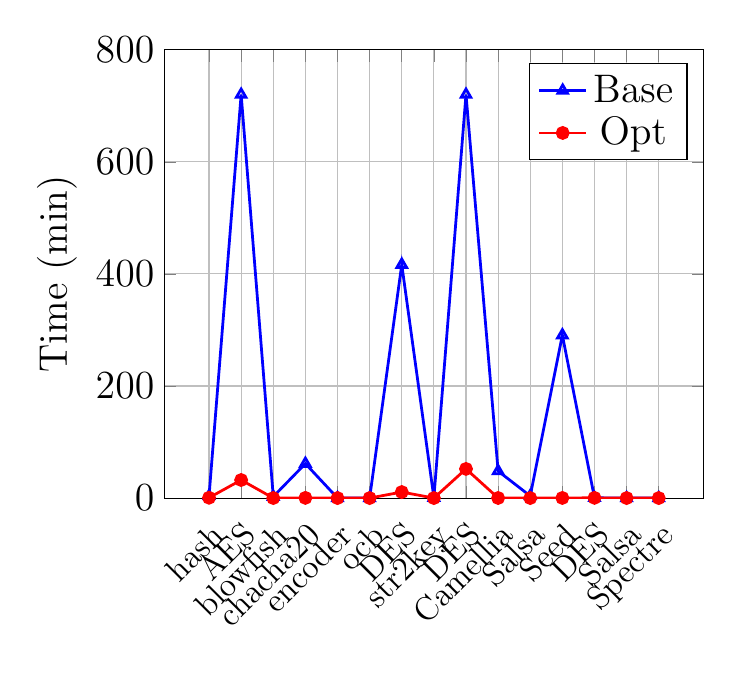
\begin{tikzpicture}
		\begin{axis}[ 
			%axis lines=left,
			ylabel= Time (min), 
			%    xlabel= Input data size(KB), 
			xtick= {1,2,3,4,5,6,7,8,9,10,11,12,13,14,15},
			xticklabel style={rotate=45, anchor=north east, inner sep=2mm},
			xticklabels = {hash,AES,blowfish,chacha20,encoder,ocb,DES,str2key,DES,Camellia,Salsa,Seed,DES,Salsa,Spectre},
			ytick = {0, 200, 400, 600, 800}, 
			yticklabels = {0, 200, 400, 600, 800}, 
			xticklabel style = {font=\large}, 
			yticklabel style = {font=\Large},
			xlabel style = {font=\Large},
			ylabel style = {font=\Large},
			ymin = 0,
			ymax = 800,
			legend style = {font=\Large}, 
			legend pos=north east, 
			grid=both]

			\addplot [line width=1pt, , color = blue, mark=triangle] plot coordinates {
					(1, 3.56) % hash
						(2, 720) % aes
						(3, 2.57) % blowfish
						(4, 61.42) % chacha20
						(5, 0.01) % encoder
						(6, 0.00) % ocb
						(7, 416.58) % des
						(8, 0.73) % str2key
						(9, 720) % des
						(10, 48.108) % camellia
						(11, 3.71) % salsa
						(12, 290.68) % seed
						(13, 0.42) % des
						(14, 0.02) % salsa
						(15, 0.00) % spectre
				};
		\label{plot:Native}
		\addplot [line width=1pt, , color = red, mark=*] plot coordinates {
			(1, 0.56)
				(2, 32.21)
				(3, 0.04)
				(4, 0.31)
				(5, 0.00)
				(6, 0.00)
				(7, 10.71)
				(8, 0.01)
				(9, 52)
				(10, 0.13)
				(11, 0.03)
				(12, 0.21)
				(13, 0.37)
				(14, 0.00)
				(15, 0.00)
		};
		\label{plot:LibOSSGX}
		\addlegendentry{Base}
		\addlegendentry{Opt}
		\end{axis}
		\end{tikzpicture}
	}
	\end{minipage}\hfill%
}
\subfigure[(b) SMT constraint size]{
	\label{fig:optb}
	\begin{minipage}{0.485\linewidth}
	\centering
		\resizebox{1.0\linewidth}{!}{
			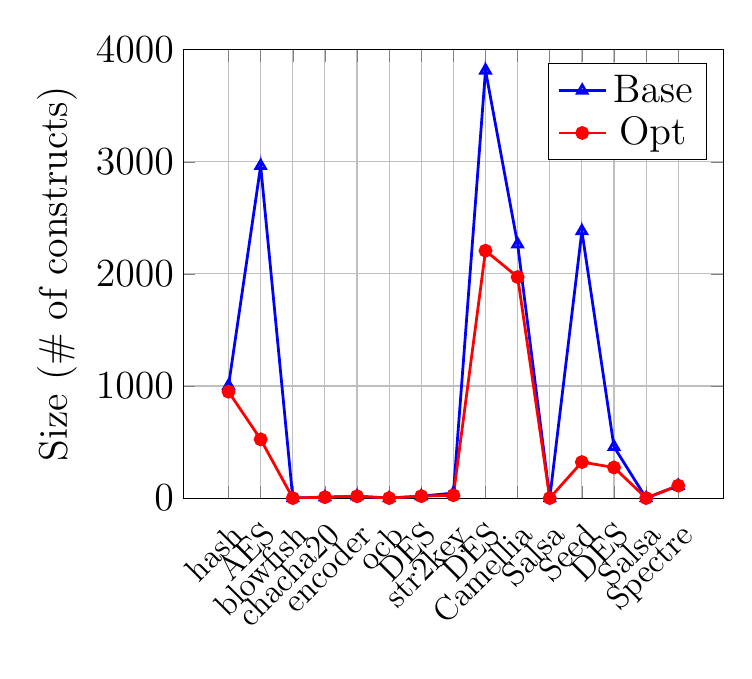
\begin{tikzpicture}
			\begin{axis}[ 
				%axis lines=left,
				ylabel= Size (\# of constructs), 
				%xlabel= Input data size(KB), 
				xtick= {1,2,3,4,5,6,7,8,9,10,11,12,13,14,15},
				xticklabel style={rotate=45, anchor=north east, inner sep=2mm},
				xticklabels = {hash,AES,blowfish,chacha20,encoder,ocb,DES,str2key,DES,Camellia,Salsa,Seed,DES,Salsa,Spectre},
				ytick = {0, 1000, 2000, 3000, 4000}, 
				yticklabels = {0, 1000, 2000, 3000, 4000}, 
				xticklabel style = {font=\large}, 
				yticklabel style = {font=\Large},
				xlabel style = {font=\Large},
				ylabel style = {font=\Large},
				ymin = 0,
				ymax = 4000,
				%ymax = 1.15, 
				legend style = {font=\Large}, 
				legend pos=north east, 
				grid=both]
				\addplot[line width=1pt, , color = blue, mark=triangle] plot coordinates {
				(1, 1003)
					(2, 2964)
					(3, 0)
					(4, 8)
					(5, 16)
					(6, 0)
					(7, 17)
					(8, 44)
					(9, 3816)
					(10, 2265)
					(11, 0)
					(12, 2382)
					(13, 457)
					(14, 0)
					(15, 111)
				};
				\label{plot:Native}
				\addplot[line width=1pt, , color = red, mark=*] plot coordinates {
					(1, 949)
					(2, 524)
					(3, 0)
					(4, 8)
					(5, 16)
					(6, 0)
					(7, 17)
					(8, 25)
					(9, 2207)
					(10, 1972)
					(11, 0)
					(12, 321)
					(13, 273)
					(14, 0)
					(15, 111)
				};
				\label{plot:LibOSSGX}
			\addlegendentry{Base}
			\addlegendentry{Opt}
			\end{axis}
			\end{tikzpicture}
		}
	\end{minipage}\hfill
}
\caption{Breakdown of Optimization Performance. Benchmarks are represented using their orders in table~\ref{tbl:benchs}.}
\label{fig:InsampleOutsample}
\label{fig:opt}
\end{figure}


\ignore{
\begin{filecontents*}{mydata.csv}
a, No-opt, Simplify and Caching, Solving Reduction, All
1, 3.56, 1.19, 1.66, 0.56 % hash
2, 720, 0,0, 32.21 % aes
3, 2.57, 0.87, 1.21, 0.04  % blowfish 
4, 61.42, 0,0, 0.31 % chacha20
5, 0.01, 0.65, 1.32, 0.00 % encoder
6, 0.00, 0.75, 1.32, 0.00 % ocb
7, 416.58, 0.85, 1.32, 10.71 % des
8, 0.73, 0.95, 1.32, 0.01 % str2key
9, 720, 0, 0, 52 % des
10, 48.108, 1.45, 1.32, 0.13 % camellia
11, 3.71, 1.45, 1.32, 0.03 % salsa
12, 290.68, 1.45, 1.32, 0.21 % seed 
13, 0.42, 1.45, 1.32, 0.37 % des
14, 0.02, 1.45, 1.32, 0.00 % salsa
15, 0.00, 1.45, 1.32, 0.00 % spectre
\end{filecontents*}

\begin{filecontents*}{cmp2.csv}
a, No-opt, Simplify and Caching, Solving Reduction, All
1, 1003, 1.19, 1.66, 949 % hash
2, 2964, 0.87, 1.21, 524 % aes
3, 0, 0.64, 1.21, 0 % blowfish 
4, 8, 0.65, 1.32, 8 % chacha20
5, 16, 0.75, 1.32, 16 % encoder
6, 0, 0.85, 1.32, 0 % ocb
7, 17, 0.95, 1.32, 17 % des
8, 44, 1.45, 1.32, 25 % str2key
9, 3816, 1.45, 1.32, 2207  % des
10, 2265, 1.45, 1.32, 1972 % camellia
11, 0, 1.45, 1.32, 0 % salsa
12, 2382, 1.45, 1.32, 321 % seed 
13, 457, 1.45, 1.32, 273 % des
14, 0, 1.45, 1.32, 0 % salsa
15, 111, 1.45, 1.32, 111 % spectre
\end{filecontents*}


\begin{figure}%[htb!]
  \centering
  \subfigure[Benchmark analysis time.]{
    \label{fig:opta}
    \scalebox{.5}{
      \begin{tikzpicture}
        \pgfplotsset{every axis legend/.append style={
          at={(0.84,0.76)}, anchor=south},every axis y label/.append style={at={(0.09,0.5)}}}
        \begin{axis}[%title=(a) Mean STD for ,xlabel=Benchmarks,
            ylabel=Time (m),xtick =data, %xticklabels={hash,AES,blowfish,chacha20,encoder,ocb}, 
            legend columns=1,legend style={font=\large},font=\large,width=8cm]
            \addplot table [x=a, y=No-opt,, col sep=comma] {mydata.csv};
            %\addplot table [x=a, y=Simplify and Caching, col sep=comma] {mydata.csv};
            %\addplot table [x=a, y=Solving Reduction, col sep=comma] {mydata.csv};
            \addplot table [x=a, y=All, col sep=comma] {mydata.csv};
            %\legend{Base, +S\&C, +SCR, All}
            \legend{Base, Opt}
        \end{axis}
      \end{tikzpicture}
      }
    }
    \subfigure[SMT constraint size.]{
    \label{fig:optb}
      \scalebox{.5}{
        \begin{tikzpicture}
          \pgfplotsset{every axis legend/.append style={
            at={(0.84,0.76)}, anchor=south},every axis y label/.append style={at={(0.09,0.5)}}}
          \begin{axis}[%title=(a) Mean STD for ,xlabel=Benchmarks,
              ylabel=Size,xtick =data, %xticklabels={hash,AES,blowfish,chacha20,encoder,ocb}, 
              legend columns=1,legend style={font=\large},font=\large,width=8cm]
              \addplot table [x=a, y=No-opt,, col sep=comma] {cmp2.csv};
              %\addplot table [x=a, y=Simplify and Caching, col sep=comma] {cmp2.csv};
              %\addplot table [x=a, y=Solving Reduction, col sep=comma] {cmp2.csv};
              \addplot table [x=a, y=All, col sep=comma] {cmp2.csv};
              %\legend{Base, +S\&C, +SCR, All}
              \legend{Base, Opt}
          \end{axis}
        \end{tikzpicture}
        }
      }
      \vspace{-1.5em}
      \caption{Breakdown of Optimization Performance. Benchmarks are represented using their orders in table~\ref{tbl:benchs}.}\label{fig:InsampleOutsample}
     \label{fig:opt}
\end{figure}
}


\begin{table}%[!tb]
\caption{Overall performance Increases from Optimization. }
%\vspace{-1em}
\label{tbl:opt}
\centering
\resizebox{\linewidth}{!}{
\begin{tabular}{ccccc}
\hline
\textbf{~~Optimization~~} &\textbf{~~Time~~}&\textbf{~~Constraints Size~~}&~~\#\textbf{.Div}~~&~~\#\textbf{.Opp}~~ \\ 
\hline
\texttt{Base} &~~~100\%~~~ &100\%    &12  &76\\ 
%\texttt{+S\&C} &~~~2400~~~ &2.13k  &8  &7\\ %2
%\texttt{+SCR} &~~~1200~~~ &1.24  &9  &10\\ %2
\texttt{Optimized} &~~~30.73\%~~~ &78.89\%  &50 &79\\ %2
\hline
%\bottomrule
\end{tabular}
}
\end{table}



\subsection{Threat to Validity}
\label{sec:threat}
Our approach considers nested speculative execution because branch 
instruction may also exist in speculative states. Since the time window 
of speculative execution is typically short, we implement the nest depth 
as configurable and set it to 2 in evaluation. Though speculative execution 
may end at arbitrary points, we demonstrate the effectiveness of our
under-approximation in the experiments. 

Another threat is from the impact 
of out-of-order execution. Out-of-order execution also reschedules memory 
accesses, which may affect the accuracy our analysis. However, considering 
both speculative execution and out-of-order execution is challenging. We 
leave it as our future work. 

We do not consider the speculative execution 
that leverages Branch Target Buffer (BTB) or Return Stack Buffer (RSB) to 
select the destinations of indirect branches. Such vulnerabilities have 
been effectively mitigated by Intel and AMD through Indirect Branch 
Prediction Barrier (IBPB) settings.

\SpecuSym analyzes LLVM IR to detect leaks caused by speculative execution. 
However, the program runtime behavior can be different due to back-end 
compiler optimization and address space layout randomization (ASLR). 
Although we have simulated the execution environment, more low-level 
details of benchmarks can further facilitate us to improve analysis 
results.



%\newpage
\section{Related Work}
\label{sec:related}

Regarding the security impact of processor speculative execution
\cite{kimuraKT1996}, Kocher et al.~\cite{KocherGGHHLMPSY19} demonstrated 
that speculative execution influences the cache state and leads to cache 
timing attacks, which motivates the design of \SpecuSym. 

To estimate cache side channels, Doychev et al.~\cite{DoychevFKMR13}
approximate cache states through concrete state abstraction. Despite the
upper bound of information leakage, the estimation offers few guidance on 
fixing the problems. Doychev et al.~\cite{DoychevK17} also shows that 
compiler optimization can remove side channels. However, it is undesirable 
for critical libraries to make the security guarantee be compiler-dependent. 

Symbolic execution~\cite{King76} has been applying to cache analysis because
of its precise reasoning and input generation natures. To quantify the 
information leakage through cache side channel, Chattopadhyay et al.
\cite{ChattopadhyayBRZ17,Chattopadhyay17} and Basu et al.~\cite{BasuC17}
developed symbolic execution methods to study dependencies between sensitive 
data and cache behaviors. Wang et al. developed CacheD~\cite{WangWLZW17} which 
aims at timing leaks through a trace-based symbolic execution. Furthermore, 
Brotzman et al.~\cite{BrotzmanLZTK2018} proposed CaSym, a symbolic reasoning 
method which supports cache analysis over multiple program paths. Considering
the cache affects from thread interleavings, Guo et al.~\cite{GuoWW18} proposed
\textsc{SymSC} to analyze cache timing leaks due to multithreading. These methods,
however, are all unaware of cache state changes under speculative execution.  


Abstract interpretation~\cite{CousotC77} has also been adopting to cache 
reasoning in terms of its scalable analysis and sound approximation. CacheS
\cite{CacheS} proposes a secret-augmented abstract domain to track program 
secrets and dependencies. It treats public data in a coarse-grained fashion 
and secret data in a finer-grained manner to balance the scalability and 
precision. However, CacheS is also unaware of the impact from speculative 
execution on cache state. Though Wu et.al~\cite{WuW19} developed a dedicated 
abstract interpretation method for worst case exectuion estimation and cache 
timing leak analysis under speculative execution, they are unable to generate 
precise inputs to diagnose the leaks in depth. 


Likewise, grey-box fuzz testing has been used in detecting Spectre-type
\cite{KocherGGHHLMPSY19} program vulnerabilities~\cite{OleksenkoTSF19}, 
exposing side channels~\cite{NilizadehNP19}, and revealing timing leaks
\cite{HeEC19}. However, these methods are either unaware of speculative 
exectution~\cite{NilizadehNP19,HeEC19} or relying on costful 
instrumentations on control flow graph. Also, due to the testing nature, 
these methods heavily count on the fuzz heuristics wheres \SpecuSym 
systematically solves for precise inputs.


To conclude, existing program analysis approaches either fail to 
generate inputs or ignore cache affects from speculative execution. 
To fill the gap, \SpecuSym models speculative execution through 
stateful symbolic execution so as to produce inputs that endorse 
the leaks. 


\section{Conclusions}
\label{sec:conclusion}


In this paper, we have presented a symbolic execution based method 
\SpecuSym for detecting cache timing leaks on running a sensitive data 
related program under speculative execution. \SpecuSym systematically 
explores the program paths and models speculative execution at conditional 
branches. By cache state modeling as well as cache behavior analysis, 
\SpecuSym uses SMT-solving to search for divergent and opposite cache 
behaviors at memory access events. Experimental results show that 
\SpecuSym can detect timing leaks under various cache settings. Comparison 
between \SpecuSym and state-of-the-art abstract interpretation based 
leak detection method shows \SpecuSym not only successfully eliminates 
false positives but also generates precise inputs for leak exposure.


\clearpage\newpage
\bibliographystyle{ACM-Reference-Format}

%\bibliographystyle{plain}
\bibliography{tapsse}


\end{document}document}
